\chapter{Levantamento bibliográfico}\label{chp:levantamento}

Este capítulo apresenta os fundamentos conceituais necessários à compreensão de
fluxos computacionais aplicados à patologia digital. A discussão não pretende
abranger exaustivamente a literatura em patologia computacional; em vez disso,
concentra-se nos conceitos que sustentam a análise metodológica desenvolvida nos
capítulos seguintes: WSIs, anotações supervisionadas, controle de qualidade,
extração de \textit{patches}, normalização de cor, segmentação semântica,
arquiteturas de aprendizagem profunda, métricas de avaliação, particionamento por
paciente, reprodutibilidade e \textit{ensembles}.

A organização do capítulo busca separar a fundamentação teórica das decisões
experimentais específicas desta dissertação. Assim, os conceitos são apresentados
inicialmente em termos gerais, com base na literatura, enquanto sua
operacionalização no fluxo proposto é detalhada no Capítulo~\ref{chp:desenvolvimento}.
Ao final, uma revisão estruturada da literatura recente examina como estudos
contemporâneos em patologia computacional oncológica tratam aspectos críticos
para a validade experimental, como qualidade dos dados, risco de vazamento,
governança, rastreabilidade e agregação de modelos.

\section{Patologia digital e WSIs}\label{sec:patologia_digital_wsi}

A patologia digital utiliza lâminas histológicas digitalizadas para visualização,
armazenamento, compartilhamento e análise computacional. Nesse contexto, a WSI
constitui a principal representação computacional da lâmina: uma imagem digital
organizada em múltiplas resoluções, capaz de preservar a arquitetura do tecido em
escala microscópica. Diferentemente de imagens convencionais em visão
computacional, uma WSI pode atingir a escala de \textit{gigapixel}, o que torna
inviável seu processamento integral como um único tensor em modelos de
aprendizagem profunda \cite{khened2021generalized,munozaguirre2020pyhist}. Por
essa razão, a análise costuma ser conduzida a partir de recortes menores,
denominados \textit{patches}, que tornam o processamento compatível com as
restrições de memória e capacidade computacional dos dispositivos disponíveis.

A \Figura{fig:wsi-patching} ilustra essa estratégia. A WSI preserva o contexto
global da lâmina, enquanto os \textit{patches} permitem operar sobre regiões
locais, adequadas ao treinamento e à inferência de modelos de segmentação. Essa
decomposição, entretanto, não deve ser compreendida apenas como uma solução
operacional. Em estudos com WSIs, a extração de \textit{patches} introduz uma
exigência de rastreabilidade: cada recorte precisa manter vínculo consistente
com a lâmina de origem, sua posição espacial, a anotação ou máscara
correspondente, o identificador do paciente e a partição experimental à qual
pertence. Sem essa associação, a relação entre imagem original, amostra
treinável e resultado avaliado torna-se frágil, dificultando a reprodução do
experimento e a interpretação científica das predições.

\begin{figure}[!htb]
    \centering
    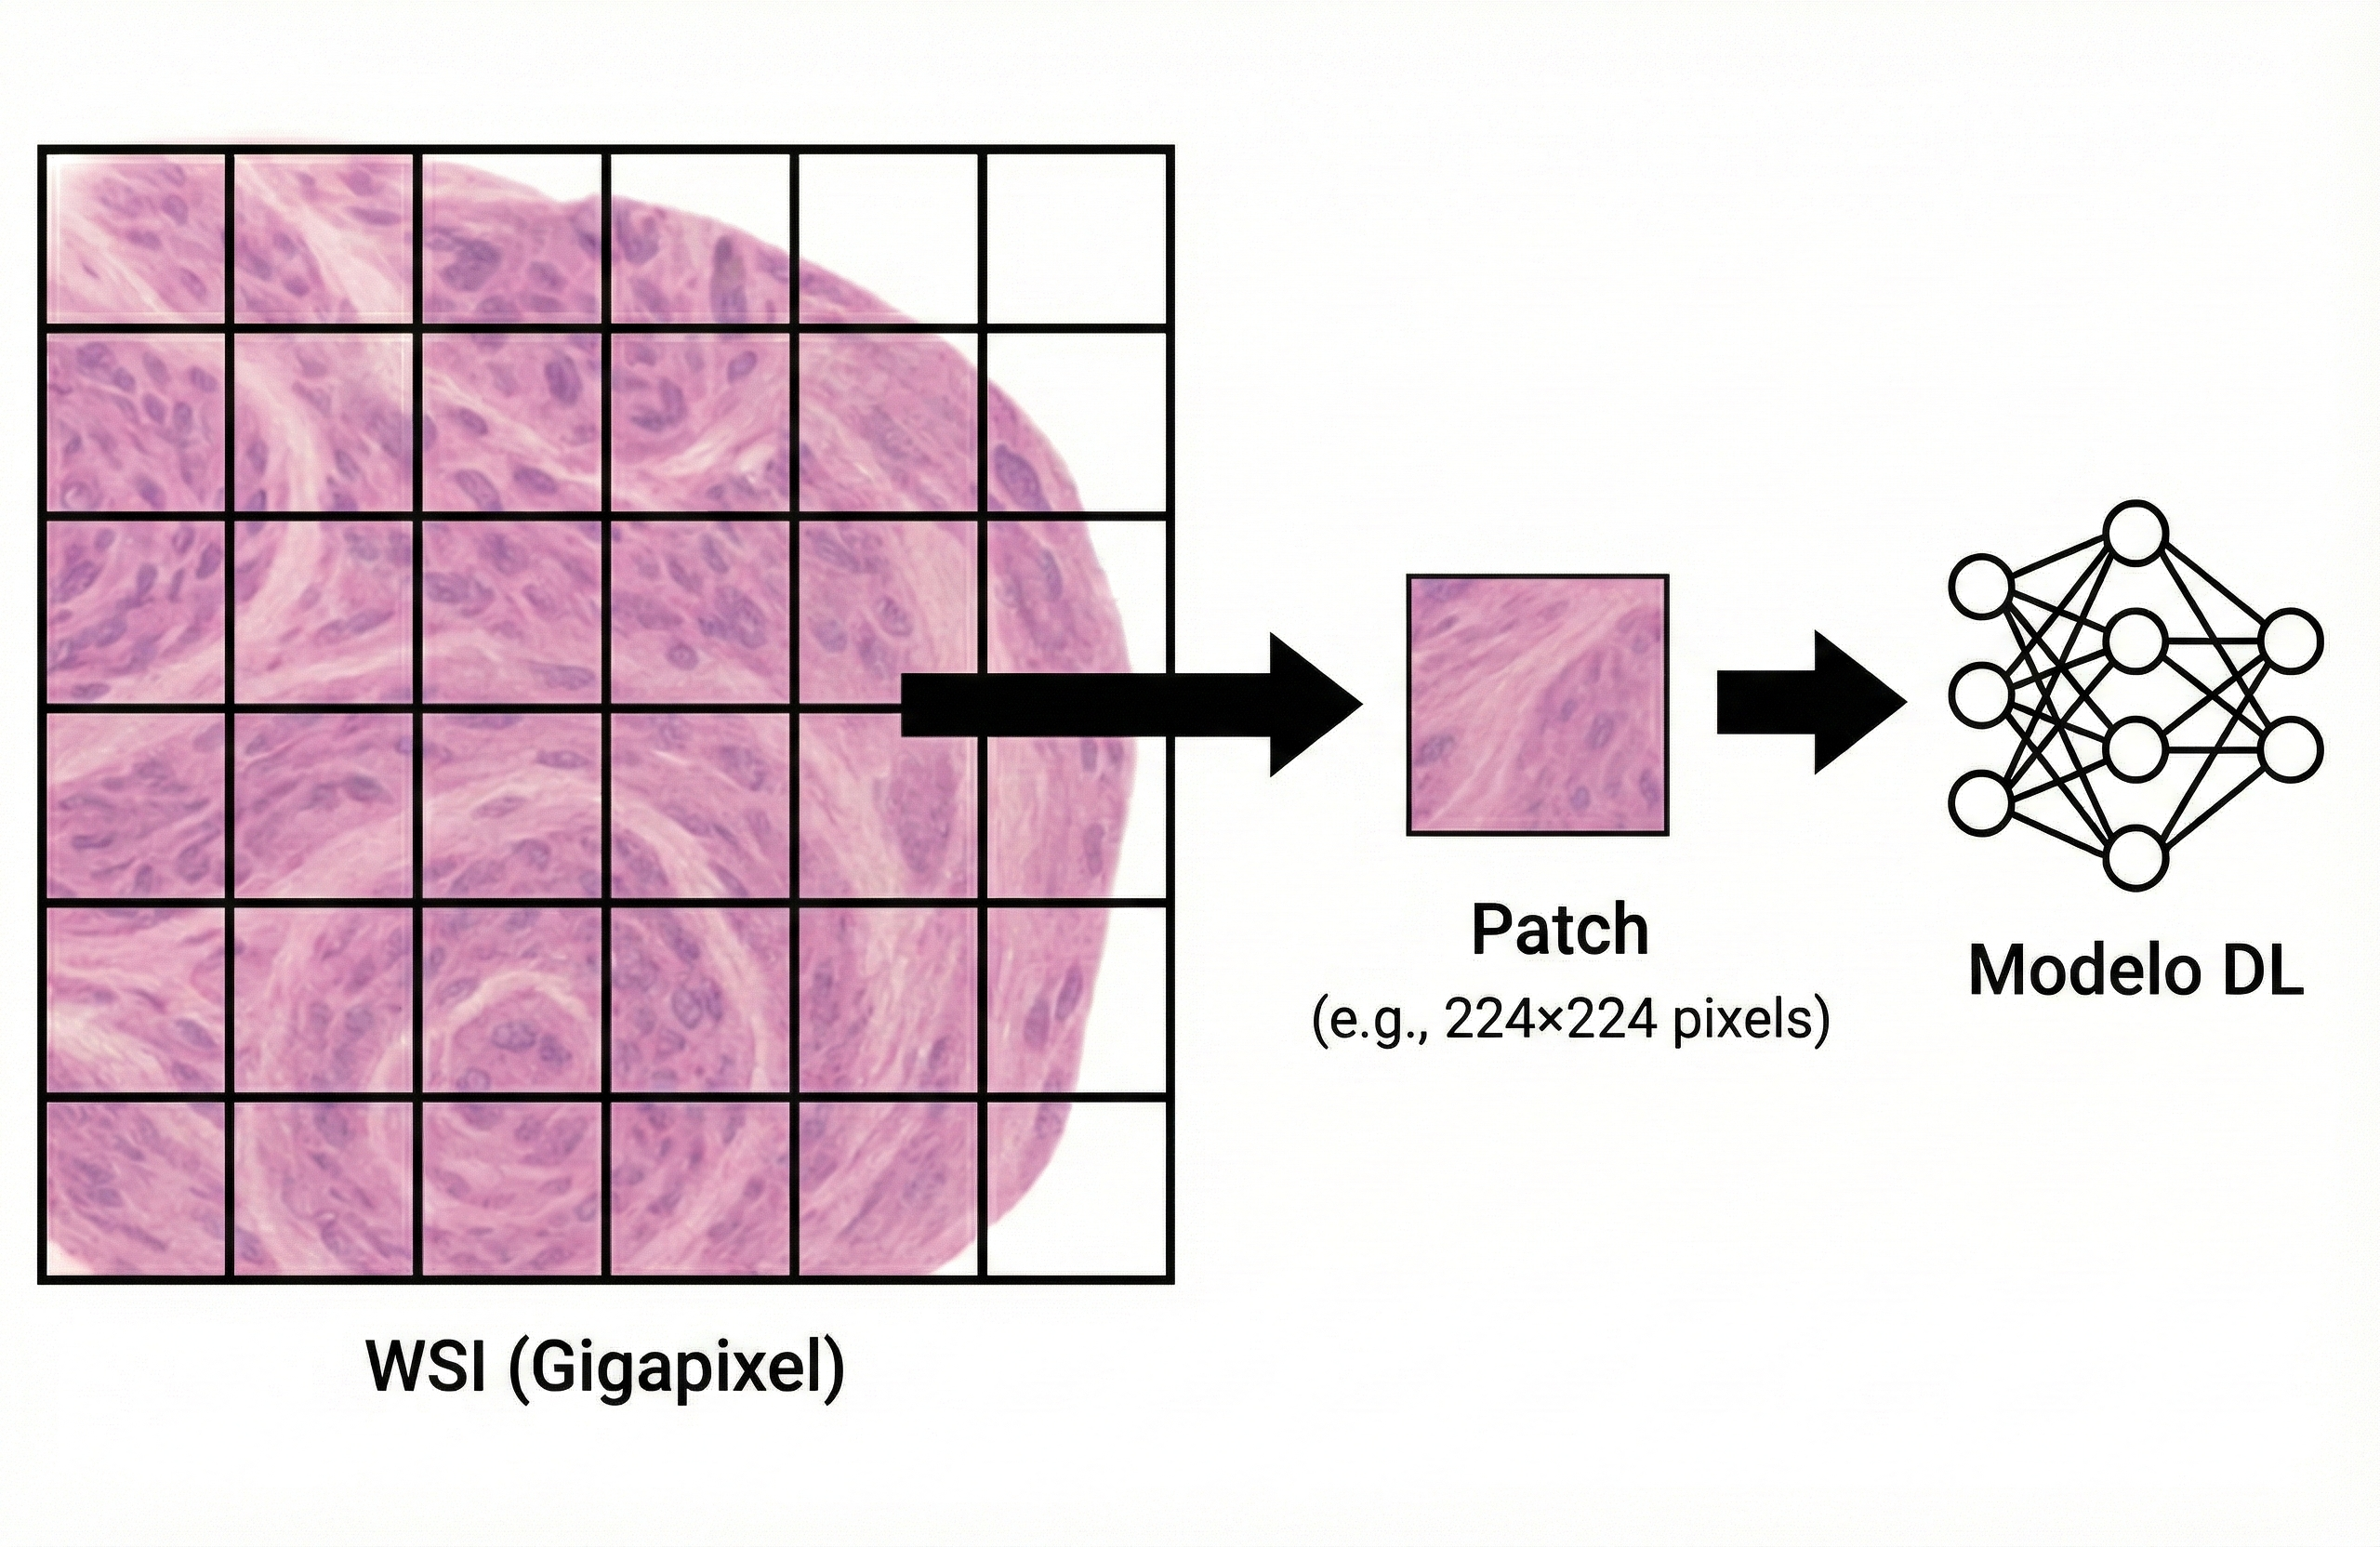
\includegraphics[width=0.92\textwidth]{figuras/WSI_schema.png}
    \caption[Estrutura de uma WSI e extração de \textit{patches}]{
    Representação conceitual de uma WSI e do processo de extração de
    \textit{patches}. A imagem completa preserva o contexto global da lâmina,
    enquanto os recortes permitem o processamento por modelos de aprendizagem
    profunda em unidades compatíveis com restrições de memória e GPU. Imagem
    gerada por ferramenta de IA (Gemini).}
    \label{fig:wsi-patching}
\end{figure}

\section{Aprendizagem profunda em patologia digital}\label{sec:ia_dl_patologia} \Sigla{Inteligência Artificial}{IA}, \Sigla{\textit{Machine Learning}}{ML} e \Sigla{\textit{Deep Learning}}{DL} representam níveis distintos de abstração em métodos computacionais baseados em dados. A IA corresponde ao campo mais amplo, voltado ao desenvolvimento de sistemas capazes de executar tarefas associadas a comportamento inteligente. O ML, por sua vez, reúne métodos que aprendem padrões a partir de exemplos, sem depender exclusivamente de regras programadas de modo explícito. O DL constitui uma subárea do ML baseada em redes neurais com múltiplas camadas, capazes de aprender representações hierárquicas diretamente dos dados \cite{goodfellow2016deep}. Essa relação é resumida na \Figura{fig:ia-ml-dl}.

\begin{figure}[!htb] \centering 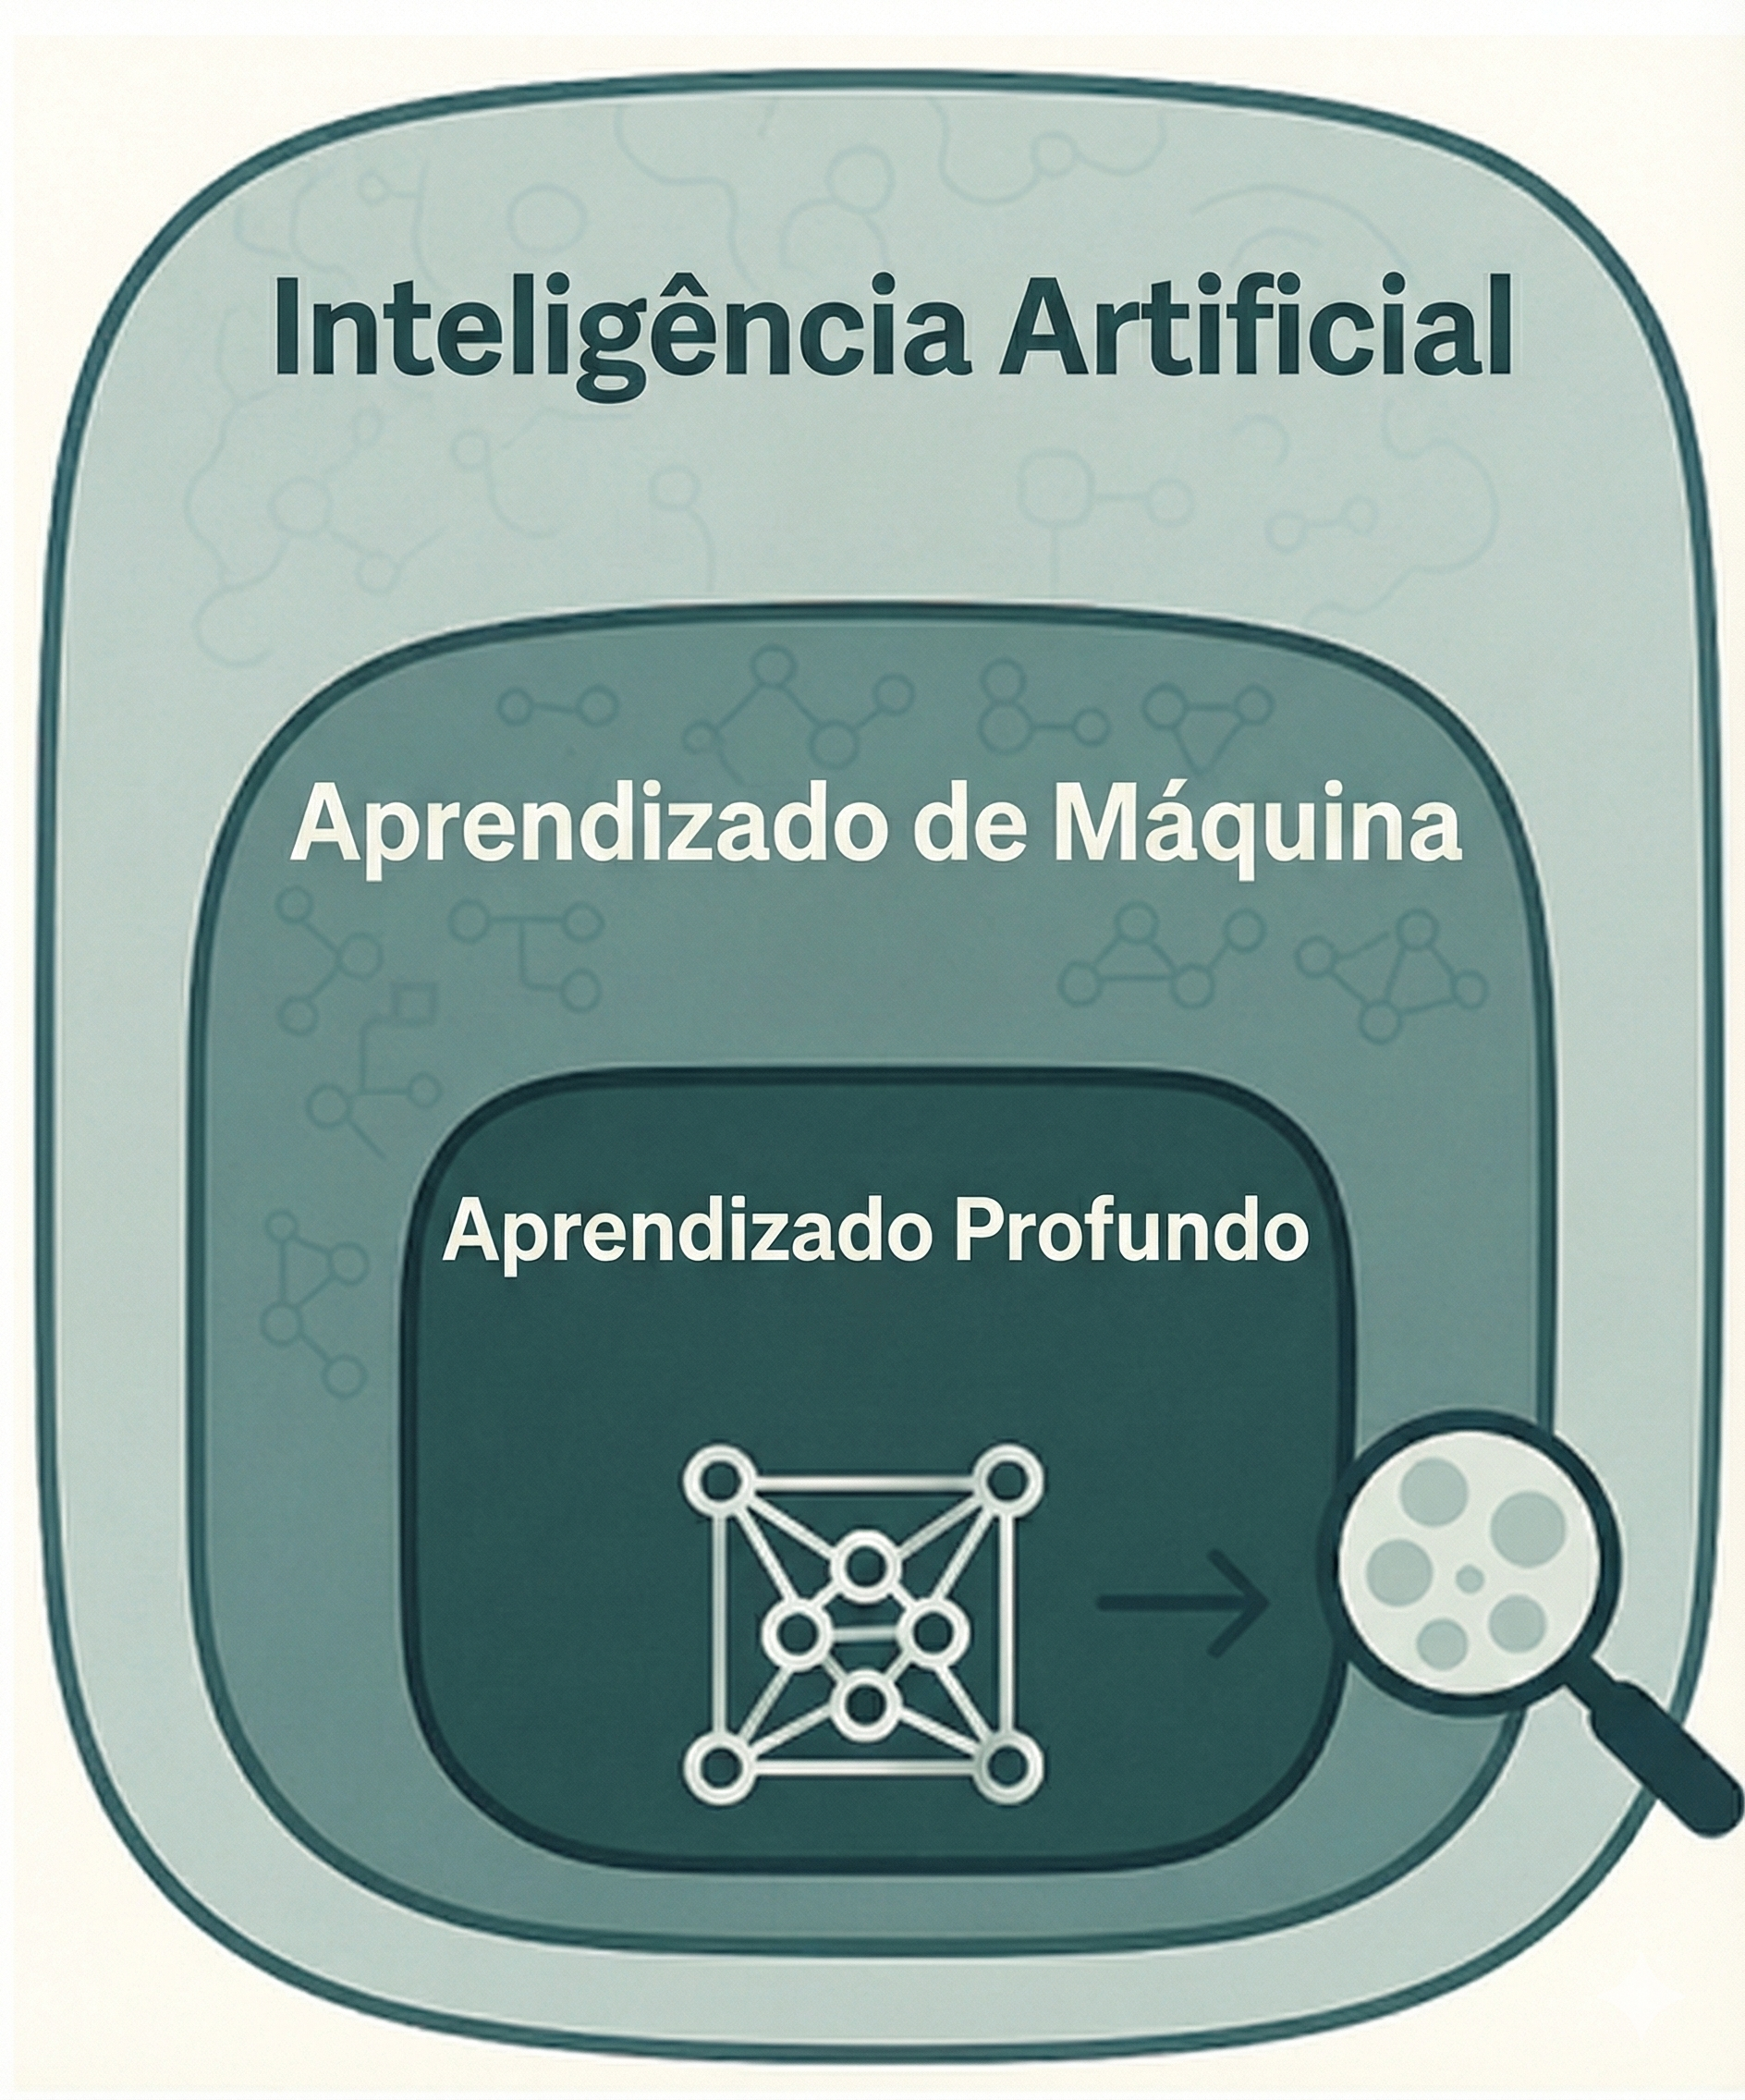
\includegraphics[width=0.58\textwidth]{figuras/AI_ML_DL.png} \caption[Hierarquia conceitual entre IA, ML e DL]{Relação hierárquica entre Inteligência Artificial, Aprendizado de Máquina e Aprendizado Profundo. Imagem gerada por ferramenta de IA (Gemini).} \label{fig:ia-ml-dl} \end{figure} 

Em aprendizagem supervisionada, o treinamento de uma rede neural pode ser descrito como um processo iterativo de ajuste de parâmetros. A cada iteração, os dados de entrada são propagados pela rede para produzir uma predição. Em seguida, essa predição é comparada com a referência anotada por meio de uma função de perda, responsável por quantificar a discrepância entre a saída esperada e a saída estimada. O erro é então retropropagado, os gradientes são calculados e o otimizador atualiza os pesos do modelo. Esse ciclo, representado na \Figura{fig:ciclo-dl}, é repetido ao longo de múltiplas épocas, até que a evolução da perda e das métricas de validação indique uma configuração adequada ao problema investigado. 

\begin{figure}[!htb] \centering 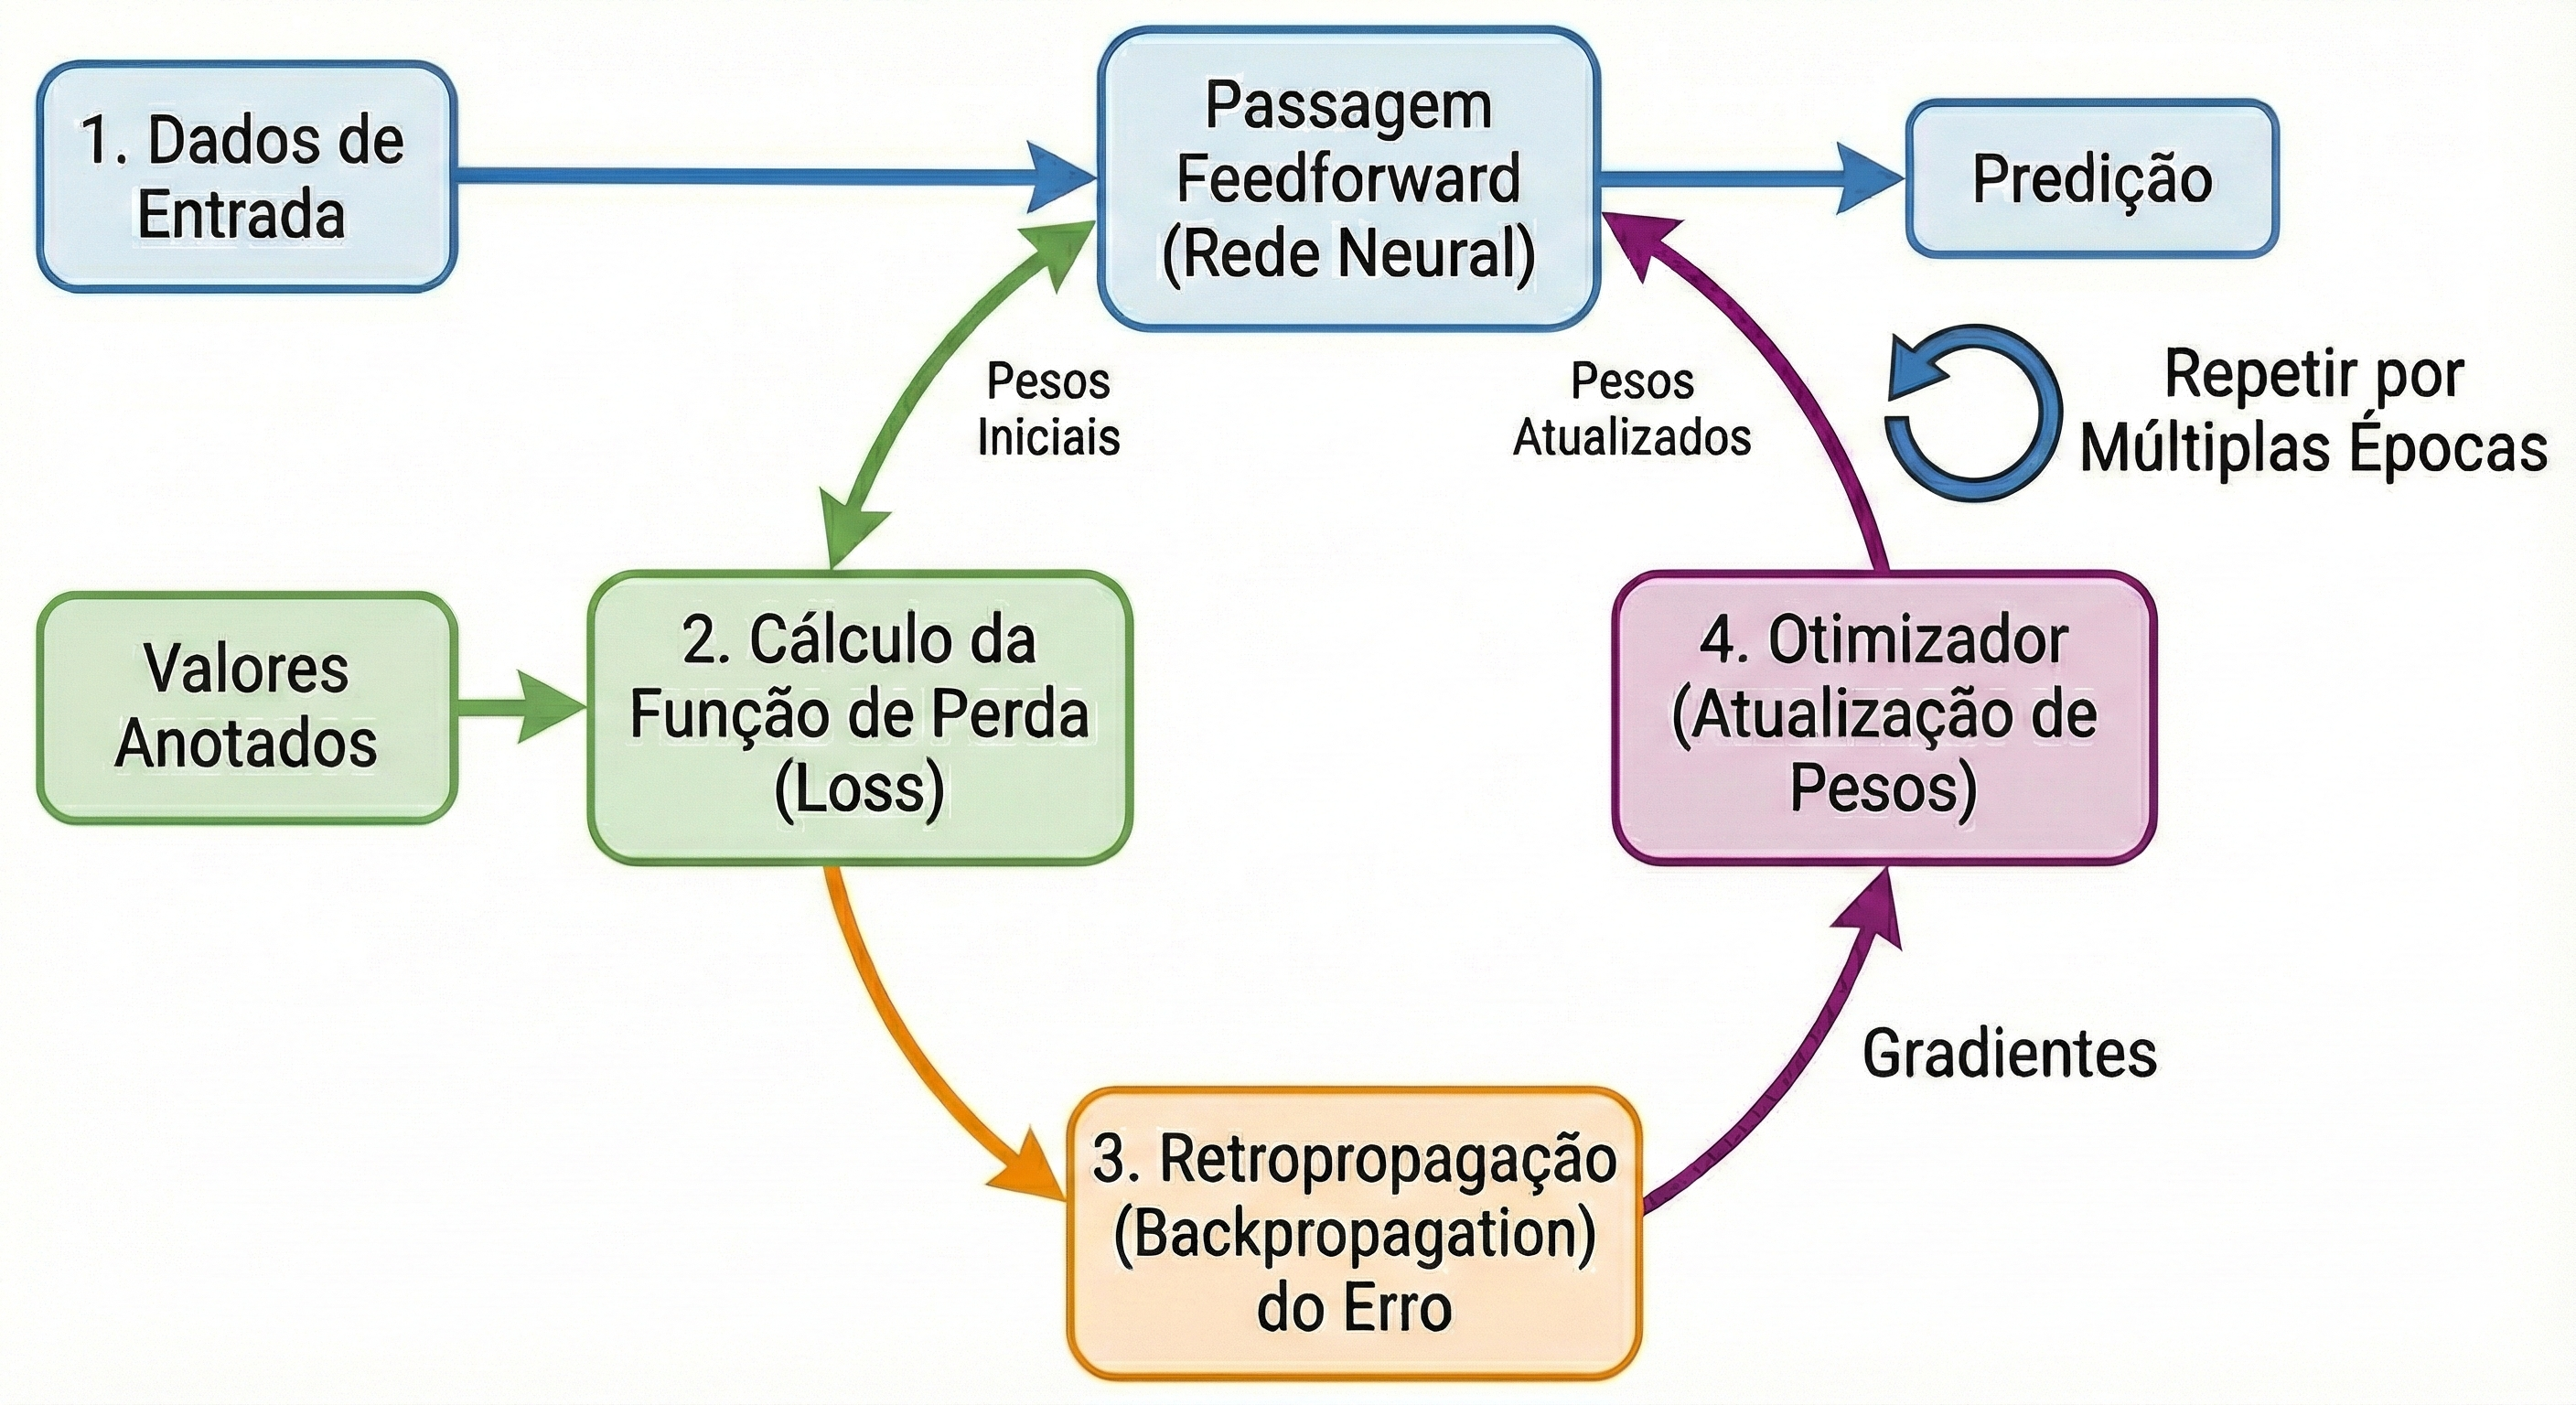
\includegraphics[width=0.78\textwidth]{figuras/DL_pipeline.png} \caption[Ciclo de treinamento de uma rede neural]{Fluxo conceitual de treinamento em aprendizagem profunda: propagação direta, comparação com a referência anotada, cálculo da função de perda, retropropagação e atualização dos pesos. Imagem gerada por ferramenta de IA (Gemini).} \label{fig:ciclo-dl} \end{figure} 

Em patologia digital, modelos de DL têm sido aplicados a diferentes tarefas de análise de imagens histológicas, incluindo classificação, detecção, segmentação semântica e análise de estruturas celulares ou teciduais \cite{deng2020deep}. No aprendizado supervisionado, essas tarefas dependem de anotações produzidas por especialistas, as quais podem delimitar tumores, tecido normal, fundo, necrose, artefatos ou outras classes de interesse. A forma como essas anotações são convertidas em rótulos, máscaras ou classes agregadas influencia diretamente a definição da tarefa computacional. Por isso, em estudos de patologia digital, é necessário explicitar quais classes histológicas são preservadas, combinadas, ignoradas ou excluídas durante a preparação dos dados, especialmente quando formulações binárias são derivadas de anotações originalmente mais detalhadas.

\section{Bases públicas em patologia digital de próstata: o caso DIAGSET} \label{sec:bases_publicas} 

Bases públicas de imagens histopatológicas desempenham papel central no avanço da patologia computacional, pois permitem comparar métodos sob protocolos documentados, reduzir barreiras de acesso a dados especializados e favorecer a reprodutibilidade de experimentos. No domínio do câncer de próstata, o DIAGSET constitui uma dessas bases de referência, por disponibilizar imagens histopatológicas associadas a diferentes níveis de anotação e avaliação diagnóstica \cite{koziarski2024diagset}.

Proposto por Koziarski et al., o DIAGSET reúne três subconjuntos complementares: DIAGSET-A, com mais de 2{,}6 milhões de \textit{patches} extraídos de 430 exames totalmente anotados; DIAGSET-B, com 4\,675 exames associados a diagnóstico binário; e DIAGSET-C, com 46 exames avaliados independentemente por nove patologistas. Essa organização permite explorar tarefas locais, baseadas em \textit{patches}, e análises em nível de exame, além de oferecer um ponto de referência para investigar a transição entre predições locais e suporte à decisão diagnóstica. 

No estudo original, a formulação binária entre câncer e não câncer foi empregada em experimentos de reconhecimento em nível de \textit{patch}, geração de mapas probabilísticos e análise em nível de lâmina. Essa estrutura torna o DIAGSET particularmente relevante para estudos que dependem de supervisão espacial, pois as anotações disponíveis permitem relacionar regiões da imagem a classes histopatológicas de interesse. Além disso, a presença de diferentes subconjuntos favorece a análise de problemas complementares, como classificação local, agregação de evidências e avaliação em nível de exame.

\begin{table}[!htb] \centering \caption{Conjunto público de imagens considerado na fundamentação da dissertação.} \label{tab:dataset_diagset} \begin{tabular}{p{2.7cm}p{3.4cm}p{5.2cm}p{4.0cm}} \toprule Conjunto & Domínio & Características principais & Relevância para estudos computacionais \\ \midrule DIAGSET & Histopatologia de câncer de próstata & Base pública composta por imagens anotadas, exames com diagnóstico binário e um subconjunto avaliado independentemente por patologistas. A porção anotada permite formular tarefas supervisionadas envolvendo câncer e tecido não canceroso. & Fornece referência pública para estudos de reconhecimento em nível de \textit{patch}, geração de mapas probabilísticos, agregação de predições e avaliação computacional em histopatologia de próstata. \\ \bottomrule \end{tabular} \end{table}

A relevância do DIAGSET também decorre de seu vínculo com um domínio clínico específico e de sua organização em múltiplas escalas de análise. Em patologia digital, essa característica é importante porque modelos treinados sobre \textit{patches} frequentemente precisam produzir evidências interpretáveis em nível de região, lâmina ou paciente. 

Assim, bases que combinam anotações locais, diagnóstico global e avaliações independentes por especialistas permitem examinar tanto o desempenho preditivo quanto a coerência entre a predição computacional e a estrutura diagnóstica do problema. Essa vantagem, entretanto, não elimina os limites de validade externa: resultados obtidos em histopatologia de próstata não podem ser extrapolados automaticamente para outros órgãos, protocolos de preparo, equipamentos de digitalização ou critérios de anotação. Por isso, estudos baseados em uma única base devem explicitar o domínio avaliado, caracterizar o conjunto de dados e evitar conclusões não verificadas em cenários histologicamente distintos. A avaliação em bases independentes permanece necessária para sustentar inferências sobre a robustez de métodos computacionais em contextos clínicos mais amplos.

\section{Pré-processamento, tecido e artefatos}\label{sec:preprocessamento_patologia} 

Antes que uma WSI seja utilizada em modelos de segmentação, é necessário distinguir regiões informativas de áreas sem conteúdo histológico útil, como fundo, vidro e regiões visualmente inválidas. Em fluxos de patologia digital, uma estratégia recorrente consiste em segmentar o tecido por meio de limiarização em uma representação de cor adequada. Entre os métodos clássicos para essa finalidade, destaca-se o método de Otsu, que seleciona automaticamente um limiar a partir do histograma da imagem \cite{otsu1979threshold}. 

De forma abstrata, a limiarização binária induzida por esse limiar pode ser escrita como: 

\begin{equation}\label{eq:otsu-threshold} g(x,y) = \begin{cases} 1, & \text{se } f(x,y) > t,\\ 0, & \text{se } f(x,y) \leq t, \end{cases} \end{equation} 

em que $f(x,y)$ representa a intensidade do pixel em uma imagem ou canal selecionado, $t$ é o limiar adotado e $g(x,y)$ é a máscara binária resultante. Nessa formulação, a máscara $g(x,y)$ permite separar, de maneira aproximada, regiões com maior probabilidade de conter tecido de áreas associadas a fundo ou ausência de material histológico. 

Máscaras obtidas apenas por limiarização podem conter ruídos, buracos internos ou pequenos componentes desconectados. Por isso, operações morfológicas são frequentemente aplicadas como etapa de refinamento. Considerando uma máscara binária $A$ e um elemento estruturante $B$, a abertura é definida como uma erosão seguida de dilatação: 

\begin{equation}\label{eq:morph-opening} A \circ B = (A \ominus B) \oplus B, \end{equation} 

enquanto o fechamento corresponde a uma dilatação seguida de erosão:

\begin{equation}\label{eq:morph-closing} A \bullet B = (A \oplus B) \ominus B. \end{equation}

Nessas expressões, $\ominus$ representa erosão e $\oplus$ representa dilatação. A abertura tende a remover componentes pequenos, protrusões finas e conexões estreitas, enquanto o fechamento tende a preencher pequenas lacunas e tornar as regiões segmentadas mais coesas \cite{gonzalez2018digital}. A \Figura{fig:morfologia} ilustra esse efeito sobre uma máscara binária.

\begin{figure}[!htb] \centering 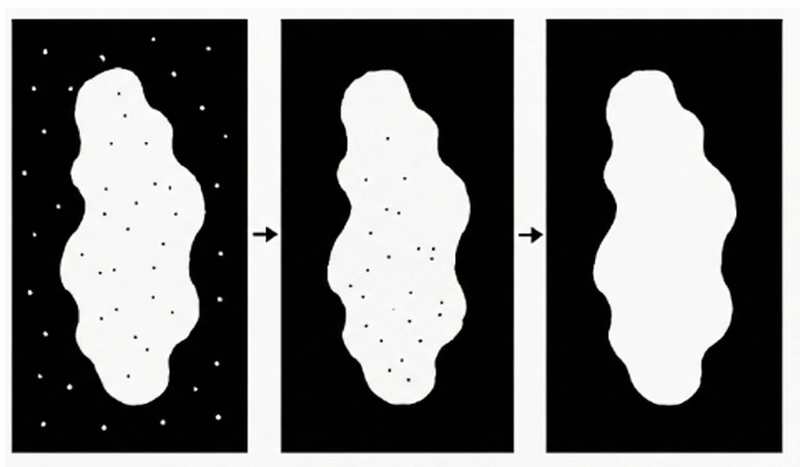
\includegraphics[width=0.78\textwidth]{figuras/morphological_operation.PNG} \caption[Operações morfológicas de abertura e fechamento]{Exemplo conceitual do efeito de abertura e fechamento sobre uma máscara binária. A abertura reduz componentes pequenos e ruídos externos, enquanto o fechamento preenche lacunas e torna a região segmentada mais coesa. Imagem gerada por ferramenta de IA (Gemini).} \label{fig:morfologia} \end{figure}

A separação entre tecido e fundo é necessária, mas insuficiente para controlar a qualidade de WSIs. Lâminas digitalizadas podem conter dobras de tecido, bolhas, marcas de caneta, regiões fora de foco, bordas da lâmina, manchas escuras e corpos estranhos. Esses artefatos introduzem sinais não biológicos que podem interferir no treinamento e na avaliação de modelos, especialmente quando se distribuem de forma desigual entre classes, scanners ou subconjuntos experimentais.

Essa preocupação motivou o desenvolvimento de ferramentas específicas de controle de qualidade em patologia digital. Um exemplo é o GrandQC, proposto por Weng et al. como uma solução automatizada para segmentação de tecido e detecção multiclasse de artefatos em WSIs coradas por hematoxilina-eosina \cite{weng2024grandqc}. O método foi validado em lâminas provenientes de diferentes departamentos de patologia, scanners e bases públicas, com o objetivo de produzir máscaras de qualidade aplicáveis ao monitoramento do preparo, da digitalização e da análise computacional de lâminas histológicas. O GrandQC segmenta tecido e regiões livres de artefatos, além de identificar classes como bolhas de ar, bordas da lâmina, regiões fora de foco, marcas de caneta, dobras de tecido, corpos estranhos e manchas escuras.

\section{Segmentação baseada em grafos em imagens histológicas} \label{sec:grafos_limpeza} A segmentação baseada em grafos oferece uma forma complementar de caracterizar regiões em imagens, especialmente quando o objetivo é separar componentes visualmente distintos sem depender apenas de limiares globais. Na formulação de \textcite{felzenszwalb2004efficient}, a imagem é representada por um grafo não direcionado $G=(V,E)$, no qual os vértices $V$ correspondem a pixels ou regiões elementares, enquanto as arestas $E$ recebem pesos associados à dissimilaridade entre elementos vizinhos. A segmentação resulta da decisão de fundir componentes ou preservar fronteiras, considerando a relação entre a variabilidade interna de cada região e a diferença observada entre regiões adjacentes.

A diferença interna de um componente $C$ é definida como:
\begin{equation}\label{eq:internal-difference} \mathrm{Int}(C)=\max_{e\in\mathrm{MST}(C,E)} w(e), \end{equation} 
em que $\mathrm{MST}$ representa a árvore geradora mínima do componente. A diferença entre dois componentes $C_1$ e $C_2$ é dada por:
\begin{equation}\label{eq:component-difference} \mathrm{Dif}(C_1,C_2)= \min_{v_i\in C_1,\,v_j\in C_2,\,(v_i,v_j)\in E} w(v_i,v_j). \end{equation}
Dois componentes são candidatos à fusão quando a diferença entre eles não excede uma medida de dissimilaridade interna ajustada pelo tamanho:
\begin{equation}\label{eq:mint} \mathrm{MInt}(C_1,C_2)= \min\left(\mathrm{Int}(C_1)+\tau(C_1),\mathrm{Int}(C_2)+\tau(C_2)\right), \quad \tau(C)=\frac{k}{|C|}. \end{equation}
Nessa formulação, $k$ controla a escala da segmentação: valores maiores tendem a produzir componentes mais amplos, enquanto valores menores favorecem regiões mais fragmentadas. 

Em histopatologia digital, essa família de métodos é relevante porque permite explorar relações locais de cor, intensidade ou textura na separação entre tecido, fundo e regiões visualmente heterogêneas. Essa característica é útil em WSIs, nas quais a variabilidade de coloração, a presença de fundo e a ocorrência de artefatos podem dificultar a definição de um único limiar global adequado para toda a lâmina. 

Um exemplo de aplicação desse princípio é o PyHIST, ferramenta de pré-processamento para imagens histológicas proposta por \textcite{munozaguirre2020pyhist}. O PyHIST utiliza segmentação baseada em grafos para produzir máscaras de tecido e orientar a seleção de \textit{tiles} com conteúdo histológico suficiente. Nesse contexto, a segmentação é empregada para distinguir regiões de primeiro plano e fundo, permitindo verificar se cada recorte satisfaz um limiar mínimo de tecido antes de ser mantido como amostra útil para análise computacional.

\begin{figure}[!htb] \centering 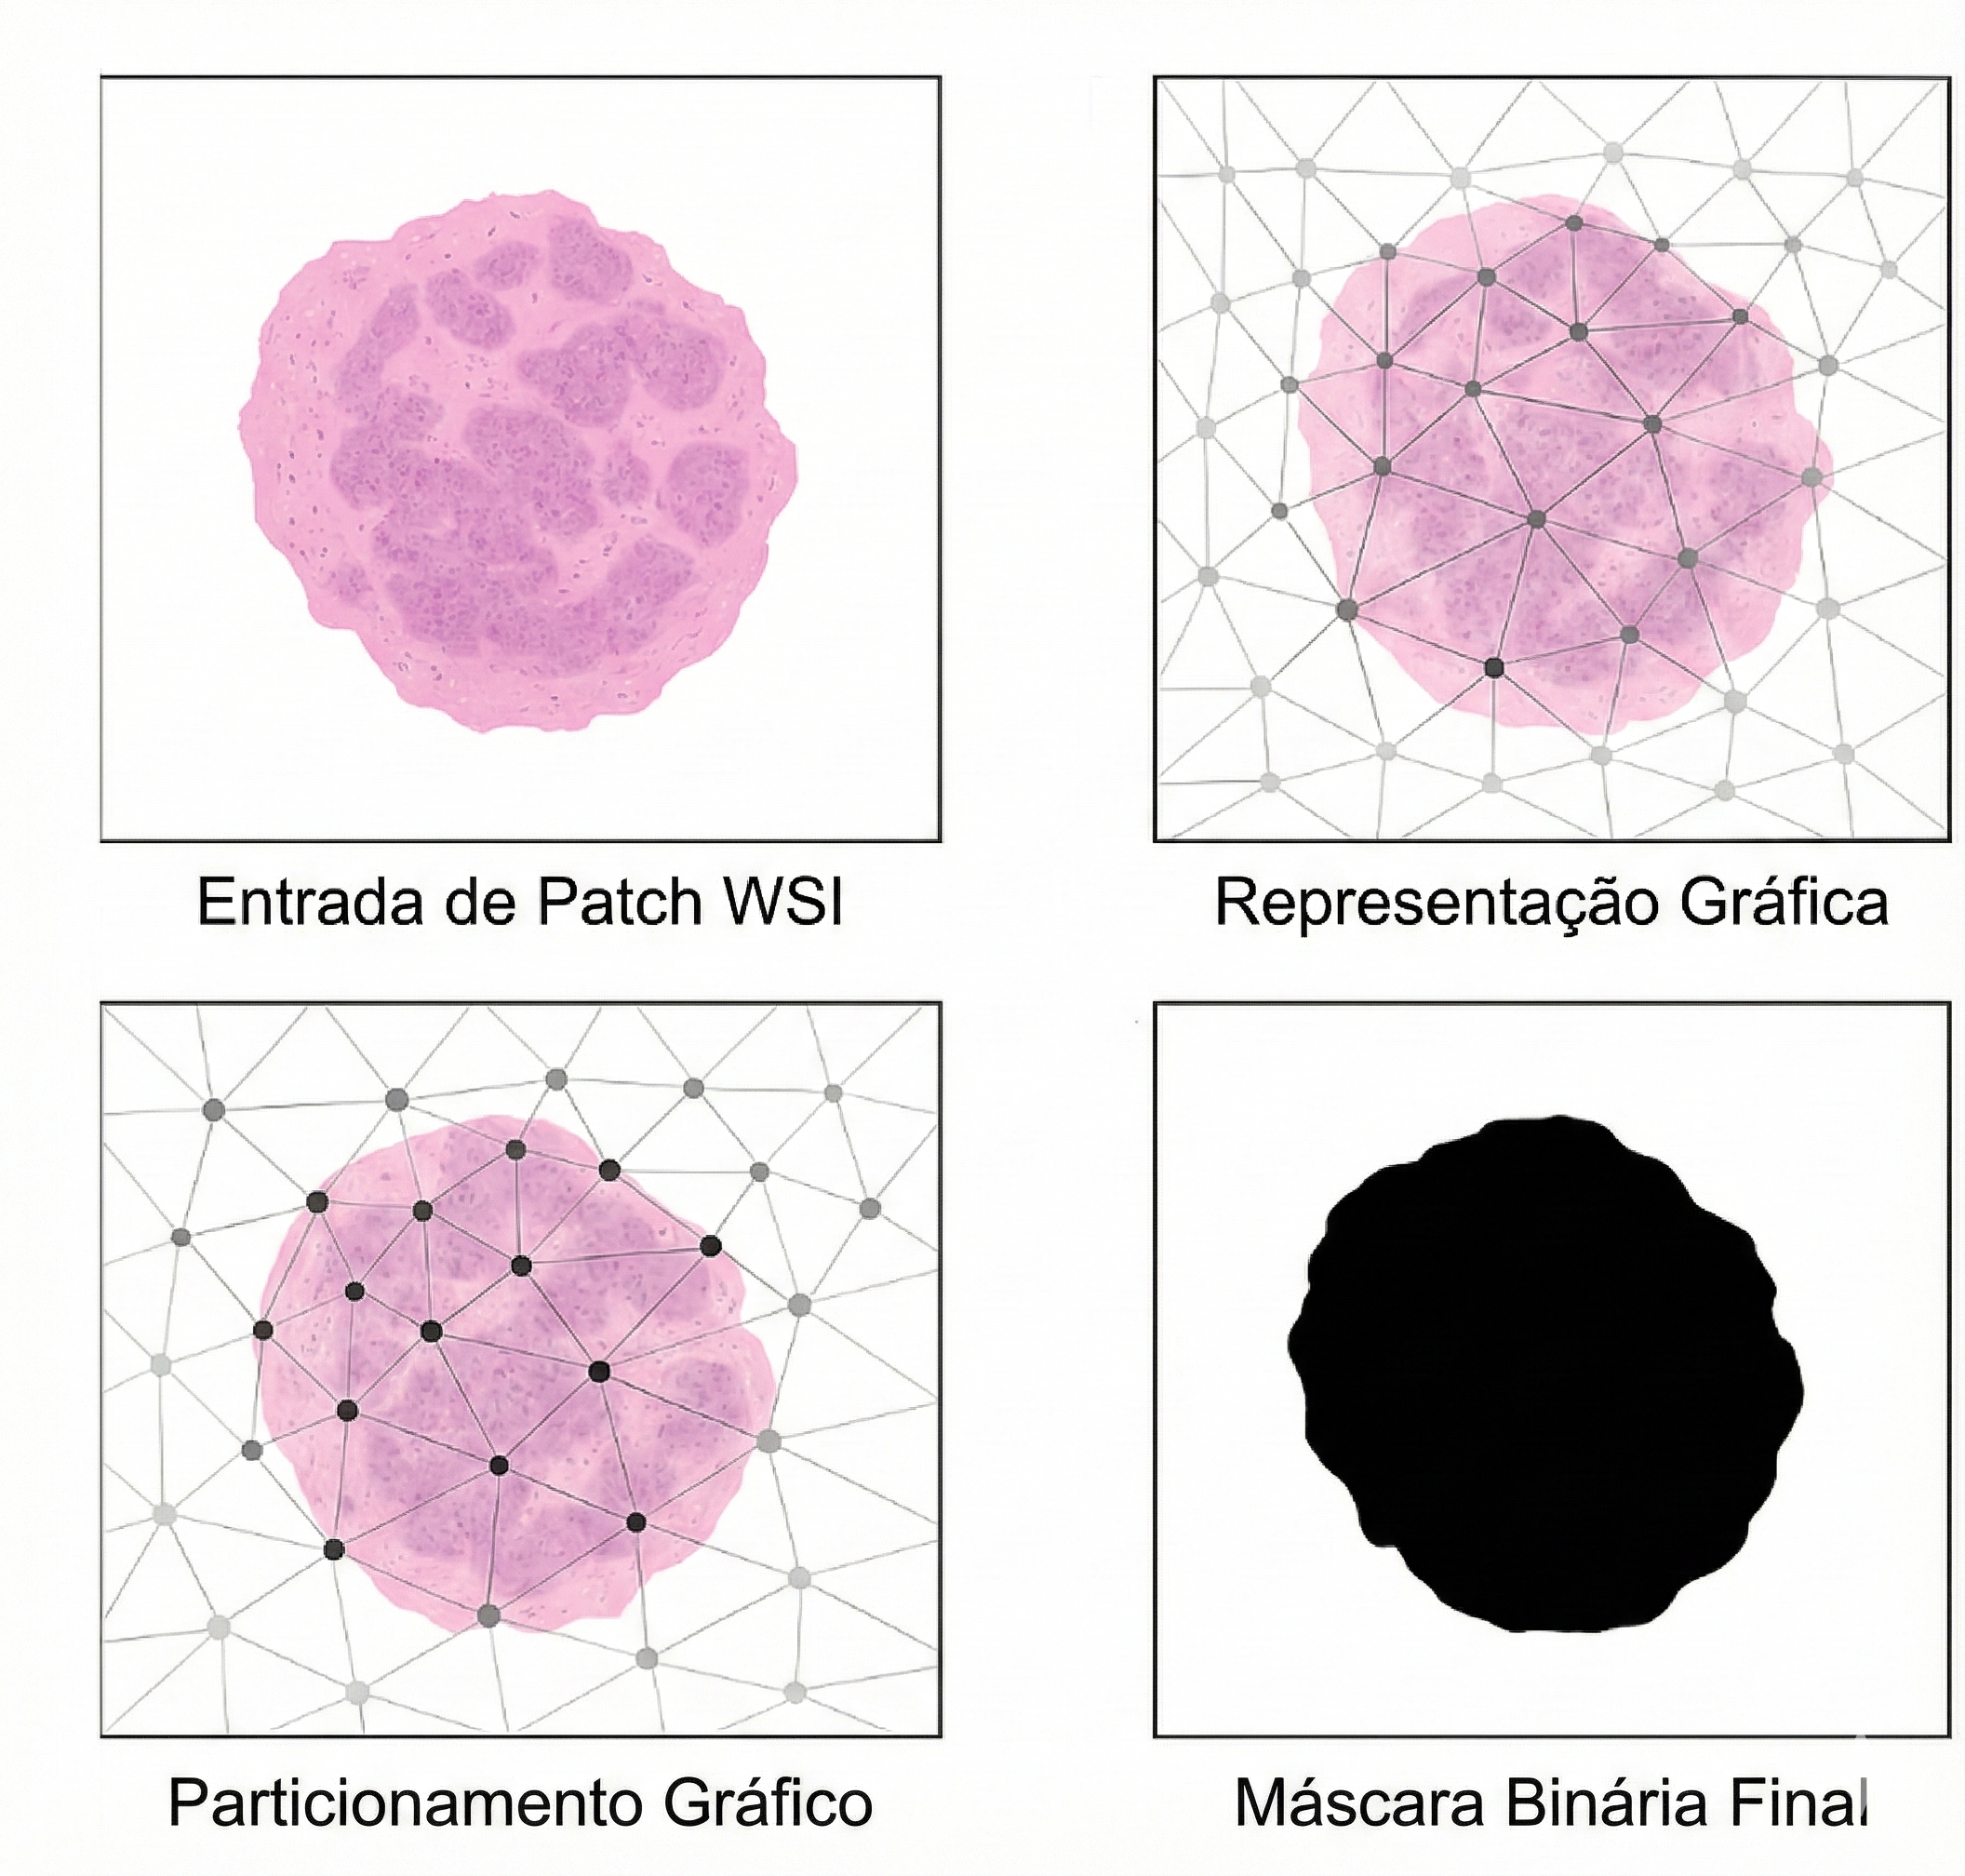
\includegraphics[width=0.88\textwidth]{figuras/graph_method.png} \caption[Segmentação de tecido baseada em grafos]{Ilustração conceitual de segmentação baseada em grafos. Pixels ou regiões elementares são representados como vértices, conectados por arestas ponderadas por dissimilaridade; a segmentação decide quais componentes devem ser fundidos e quais fronteiras devem ser preservadas. Imagem gerada por ferramenta de IA (Gemini).} \label{fig:graph-method} \end{figure}

\section{Normalização de cor}\label{sec:normalizacao_cor} 

A coloração por hematoxilina-eosina pode variar entre laboratórios, scanners, protocolos de preparo, lotes de reagentes e condições de digitalização. Essa variabilidade altera a aparência visual das lâminas e pode modificar características extraídas das imagens, levando modelos de aprendizagem profunda a associar diferenças técnicas a padrões morfológicos de interesse \cite{tellez2019augmentation,duenweg2023scanner}. Nesse contexto, a normalização de cor busca reduzir variações cromáticas não biológicas e tornar mais consistente a comparação entre amostras processadas sob condições distintas.

Uma estratégia clássica é a normalização de Reinhard, na qual uma imagem de origem é transformada de modo a aproximar suas estatísticas de cor das estatísticas de uma imagem-alvo. Para um canal $c$, a transformação pode ser escrita como: 
\begin{equation}\label{eq:reinhard-norm} I'_c = \frac{I_c-\mu_{s,c}}{\sigma_{s,c}}\sigma_{t,c}+\mu_{t,c}, \end{equation} 
em que $I_c$ representa a intensidade do canal na imagem de origem, $\mu_{s,c}$ e $\sigma_{s,c}$ são, respectivamente, a média e o desvio padrão da imagem de origem nesse canal, e $\mu_{t,c}$ e $\sigma_{t,c}$ são as estatísticas correspondentes da imagem-alvo \cite{reinhard2001color}. Essa formulação ajusta a distribuição de cores da imagem de origem, mas não modela explicitamente a contribuição dos corantes histológicos. 

Em imagens histológicas coradas por hematoxilina-eosina, abordagens baseadas em separação de corantes representam a imagem em termos de densidade óptica e estimam a contribuição de cada corante. Métodos como os propostos por Ruifrok, Macenko e Vahadane exploram essa ideia para decompor ou normalizar a aparência das lâminas, aproximando imagens obtidas sob diferentes condições a uma representação cromática mais comparável \cite{ruifrok2001quantification,macenko2009method,vahadane2016structure}. Uma forma simplificada de densidade óptica é: 
\begin{equation}\label{eq:od} \mathrm{OD}=-\log\left(\frac{I+\epsilon}{I_0}\right), \end{equation} 
em que $I$ é a intensidade observada, $I_0$ é a intensidade de referência e $\epsilon$ é um termo de estabilização numérica. Essa transformação aproxima a relação entre intensidade observada e absorção de luz pelos corantes, permitindo tratar diferenças de coloração em um espaço mais adequado à análise histológica.

\begin{figure}[!htb] \centering \begin{subfigure}{0.18\textwidth} \centering 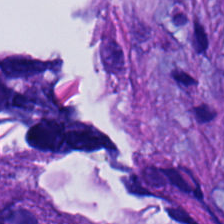
\includegraphics[width=\linewidth]{figuras/original_patch.png} \caption{Original} \end{subfigure}\hfill \begin{subfigure}{0.18\textwidth} \centering 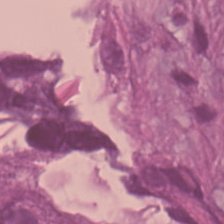
\includegraphics[width=\linewidth]{figuras/reinhard_patch.png} \caption{Reinhard} \end{subfigure}\hfill \begin{subfigure}{0.18\textwidth} \centering 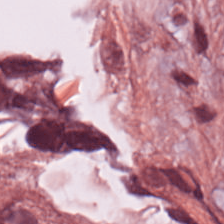
\includegraphics[width=\linewidth]{figuras/macenko_patch.png} \caption{Macenko} \end{subfigure}\hfill \begin{subfigure}{0.18\textwidth} \centering 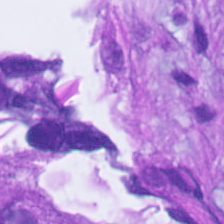
\includegraphics[width=\linewidth]{figuras/ruifrok_patch.png} \caption{Ruifrok} \end{subfigure}\hfill \begin{subfigure}{0.18\textwidth} \centering 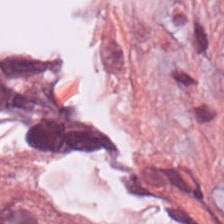
\includegraphics[width=\linewidth]{figuras/vahadane_patch.png} \caption{Vahadane} \end{subfigure} \caption[Exemplos de normalização de cor]{Exemplos visuais de métodos de normalização de cor em imagens histológicas. A figura ilustra diferenças qualitativas entre a imagem original e versões normalizadas por Reinhard, Macenko, Ruifrok e Vahadane.} \label{fig:normalizacao-exemplos} \end{figure}

\section{Aumento de dados}\label{sec:aumento_dados} 

O aumento de dados consiste em aplicar transformações às amostras de treinamento com o objetivo de expor o modelo a variações plausíveis do domínio, sem alterar o significado do rótulo ou da máscara associada. Em histopatologia, essa etapa é particularmente relevante porque a orientação do tecido raramente possui significado absoluto, enquanto textura, foco, ruído e coloração podem variar por razões técnicas relacionadas ao preparo da lâmina, ao scanner e ao processo de digitalização. Assim, rotações, espelhamentos, pequenas perturbações locais e variações cromáticas podem contribuir para reduzir a dependência de padrões acidentais presentes no conjunto de treino. 

A finalidade do aumento de dados não é produzir novas observações biológicas, mas tornar o treinamento menos sensível a variações compatíveis com o processo de aquisição das imagens. Para isso, as transformações devem preservar a correspondência entre imagem e anotação: qualquer operação espacial aplicada ao \textit{patch} precisa ser aplicada de forma equivalente à respectiva máscara de segmentação. Em tarefas supervisionadas, essa consistência é essencial para evitar desalinhamentos entre entrada e referência, os quais comprometeriam o cálculo da função de perda e a interpretação das métricas. 

Bibliotecas como \textit{Albumentations} são adequadas para esse cenário por permitirem compor transformações geométricas e fotométricas de maneira eficiente e consistente entre imagens e anotações \cite{buslaev2020albumentations,dossantos2023augmentation,shorten2019survey}. Essas transformações podem incluir espelhamentos, rotações, desfoque, perturbações cromáticas e estratégias de oclusão parcial, desde que sejam compatíveis com a variabilidade esperada do domínio e não introduzam alterações incompatíveis com a interpretação histopatológica. 

\begin{figure}[!htb] \centering \begin{subfigure}{0.24\textwidth} 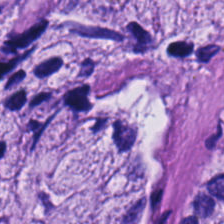
\includegraphics[width=\linewidth]{figuras/example_original.png} \caption{Original} \end{subfigure}\hfill \begin{subfigure}{0.24\textwidth} 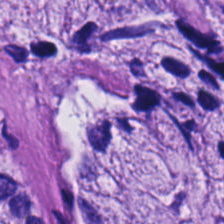
\includegraphics[width=\linewidth]{figuras/example_HF.png} \caption{Espelho horizontal} \end{subfigure}\hfill \begin{subfigure}{0.24\textwidth} 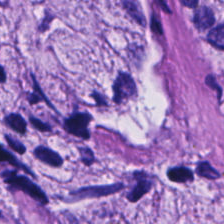
\includegraphics[width=\linewidth]{figuras/example_VF.png} \caption{Espelho vertical} \end{subfigure}\hfill \begin{subfigure}{0.24\textwidth} 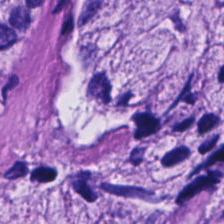
\includegraphics[width=\linewidth]{figuras/example_RR.png} \caption{Rotação} \end{subfigure} \vspace{0.4em} \begin{subfigure}{0.24\textwidth} 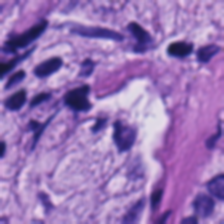
\includegraphics[width=\linewidth]{figuras/example_GB.png} \caption{Desfoque} \end{subfigure}\hfill \begin{subfigure}{0.24\textwidth} 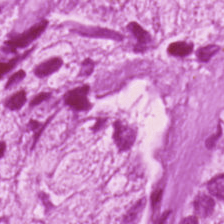
\includegraphics[width=\linewidth]{figuras/example_HED.png} \caption{Variação HED} \end{subfigure}\hfill \begin{subfigure}{0.24\textwidth} 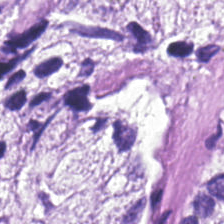
\includegraphics[width=\linewidth]{figuras/example_HSV.png} \caption{Variação HSV} \end{subfigure}\hfill \begin{subfigure}{0.24\textwidth} 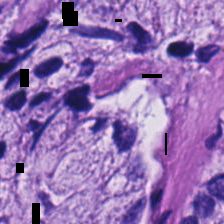
\includegraphics[width=\linewidth]{figuras/example_coarse_dropout.png} \caption{Descarte de região} \end{subfigure}\hfill \caption[Exemplos de aumento de dados]{Exemplos qualitativos de transformações de aumento de dados em imagens histológicas. As transformações ilustram variações geométricas e fotométricas que podem ser aplicadas ao \textit{patch} e, quando houver operação espacial, também à máscara correspondente.} \label{fig:augmentation-exemplos} \end{figure}


\section{Otimização e função de perda}\label{sec:otimizacao_loss} 

O treinamento supervisionado de redes neurais pode ser entendido como a minimização de uma função de perda, isto é, uma medida da discrepância entre a predição do modelo e a referência anotada. Essa função transforma o problema de aprendizagem em um problema de otimização: a cada iteração, os parâmetros da rede são ajustados para reduzir o erro observado no conjunto de treinamento, com o objetivo de favorecer a generalização para dados não utilizados no ajuste dos pesos \cite{goodfellow2016deep}. 

Em segmentação semântica, a função de perda deve considerar tanto a classificação pixel a pixel quanto a sobreposição espacial entre a máscara prevista e a máscara de referência. A entropia cruzada binária penaliza erros locais de classificação em cada pixel, enquanto termos baseados no coeficiente de Dice favorecem a concordância espacial entre regiões segmentadas. Essa combinação é particularmente útil em tarefas biomédicas desbalanceadas, nas quais a classe de interesse pode ocupar uma fração reduzida da imagem \cite{sudre2017generalised}.

Formulações híbridas combinam esses dois objetivos em uma única função de perda. Uma forma adotada em segmentação de imagens histológicas combina um termo de entropia cruzada binária com termos Dice associados ao fundo e ao primeiro plano, como descrito por \textcite{khened2021generalized}. De forma geral, essa composição pode ser escrita como: 

\begin{equation}\label{eq:hybrid-loss} \mathcal{L} = \alpha \mathcal{L}_{\mathrm{BCE}} + \beta \mathcal{L}_{\mathrm{Dice,bg}} + \gamma \mathcal{L}_{\mathrm{Dice,fg}}, \end{equation} 
em que $\mathcal{L}_{\mathrm{BCE}}$ representa o termo de entropia cruzada binária, $\mathcal{L}_{\mathrm{Dice,bg}}$ e $\mathcal{L}_{\mathrm{Dice,fg}}$ representam os termos Dice para fundo e primeiro plano, respectivamente, e $\alpha$, $\beta$ e $\gamma$ controlam a contribuição relativa de cada componente. Essa formulação permite equilibrar a penalização de erros pixel a pixel com a qualidade global da segmentação, reduzindo a dependência de uma única medida de erro. 

A otimização dos parâmetros do modelo é realizada por algoritmos iterativos que atualizam os pesos a partir dos gradientes da função de perda. Nesse contexto, um dos desafios é definir não apenas a direção da atualização, mas também sua escala para cada parâmetro ao longo do treinamento. Entre os otimizadores adaptativos, o Adam estima médias móveis do primeiro e do segundo momento dos gradientes, ajustando a magnitude das atualizações de forma individualizada \cite{kingma2015adam}. De forma simplificada, essa atualização pode ser representada por: 
\begin{equation}\label{eq:adam-update} \theta_{t+1} = \theta_t - \eta \frac{\hat{m}_t}{\sqrt{\hat{v}_t}+\epsilon}, \end{equation} 
em que $\theta_t$ representa os parâmetros no passo $t$, $\eta$ é a taxa de aprendizado, $\hat{m}_t$ e $\hat{v}_t$ são as estimativas corrigidas do primeiro e do segundo momento dos gradientes, e $\epsilon$ é um termo de estabilidade numérica. 

Além da atualização dos pesos, o treinamento de redes profundas costuma incluir mecanismos de regularização para reduzir sobreajuste. O AdamW parte da lógica adaptativa do Adam, mas modifica a forma como o decaimento de peso é aplicado. Em implementações baseadas em regularização $L_2$, a penalização proporcional à norma quadrática dos parâmetros é incorporada à função de perda; no AdamW, em contrapartida, o decaimento de peso é desacoplado do gradiente da perda e aplicado diretamente aos parâmetros \cite{loshchilov2019decoupled}:

\begin{equation}\label{eq:adamw-update} \theta_{t+1} = \theta_t - \eta \frac{\hat{m}_t}{\sqrt{\hat{v}_t}+\epsilon} - \eta\lambda\theta_t, \end{equation}

em que $\lambda$ controla a intensidade do decaimento de peso. Essa separação torna explícito o papel regularizador do decaimento de peso e evita que ele seja misturado à estimativa adaptativa dos gradientes. 

Outro componente importante da otimização é a evolução da taxa de aprendizado ao longo do treinamento. Em abordagens tradicionais, essa evolução é controlada por um escalonador, que reduz ou ajusta $\eta$ segundo uma agenda predefinida, frequentemente dependente do número total de passos. Métodos \textit{schedule-free} foram propostos como alternativa a esse desenho: em vez de exigir uma agenda explícita, combinam interpolação e média iterativa dos parâmetros, buscando substituir parte do papel desempenhado pelos escalonadores e mantendo a taxa de aprendizado como hiperparâmetro central \cite{defazio2024road}. 

Em conjunto, aumento de dados, função de perda, otimizador e taxa de aprendizado definem as condições sob as quais o modelo observa variações dos dados, calcula o erro e atualiza seus parâmetros. Por essa razão, esses elementos devem ser descritos de forma explícita em estudos de segmentação supervisionada, especialmente quando diferentes arquiteturas, estratégias de pré-processamento ou critérios de seleção de modelos são comparados sob um mesmo protocolo experimental.

\section{Segmentação semântica e arquiteturas neurais}
\label{sec:segmentacao_arquiteturas}

Esta seção introduz o conceito de segmentação semântica e descreve como
diferentes arquiteturas neurais podem ser usadas para transformar uma imagem de
entrada em uma máscara de predição pixel a pixel.

\subsection{Segmentação semântica} \label{subsec:segmentacao_semantica} 

A segmentação semântica consiste em atribuir uma classe a cada pixel de uma imagem. Diferentemente da classificação, que produz um rótulo global para a imagem, a segmentação preserva a estrutura espacial da predição. Em uma tarefa binária de câncer, a saída esperada é uma máscara na qual pixels associados à região tumoral pertencem à classe positiva, enquanto os demais pixels pertencem à classe negativa. Essa formulação é particularmente relevante em patologia digital, pois permite não apenas indicar a presença de câncer, mas também estimar sua localização e extensão espacial. 

A \Figura{fig:semantic-segmentation} ilustra a relação entre imagem de entrada, classes de interesse e máscara predita. 

\begin{figure}[!htb] \centering 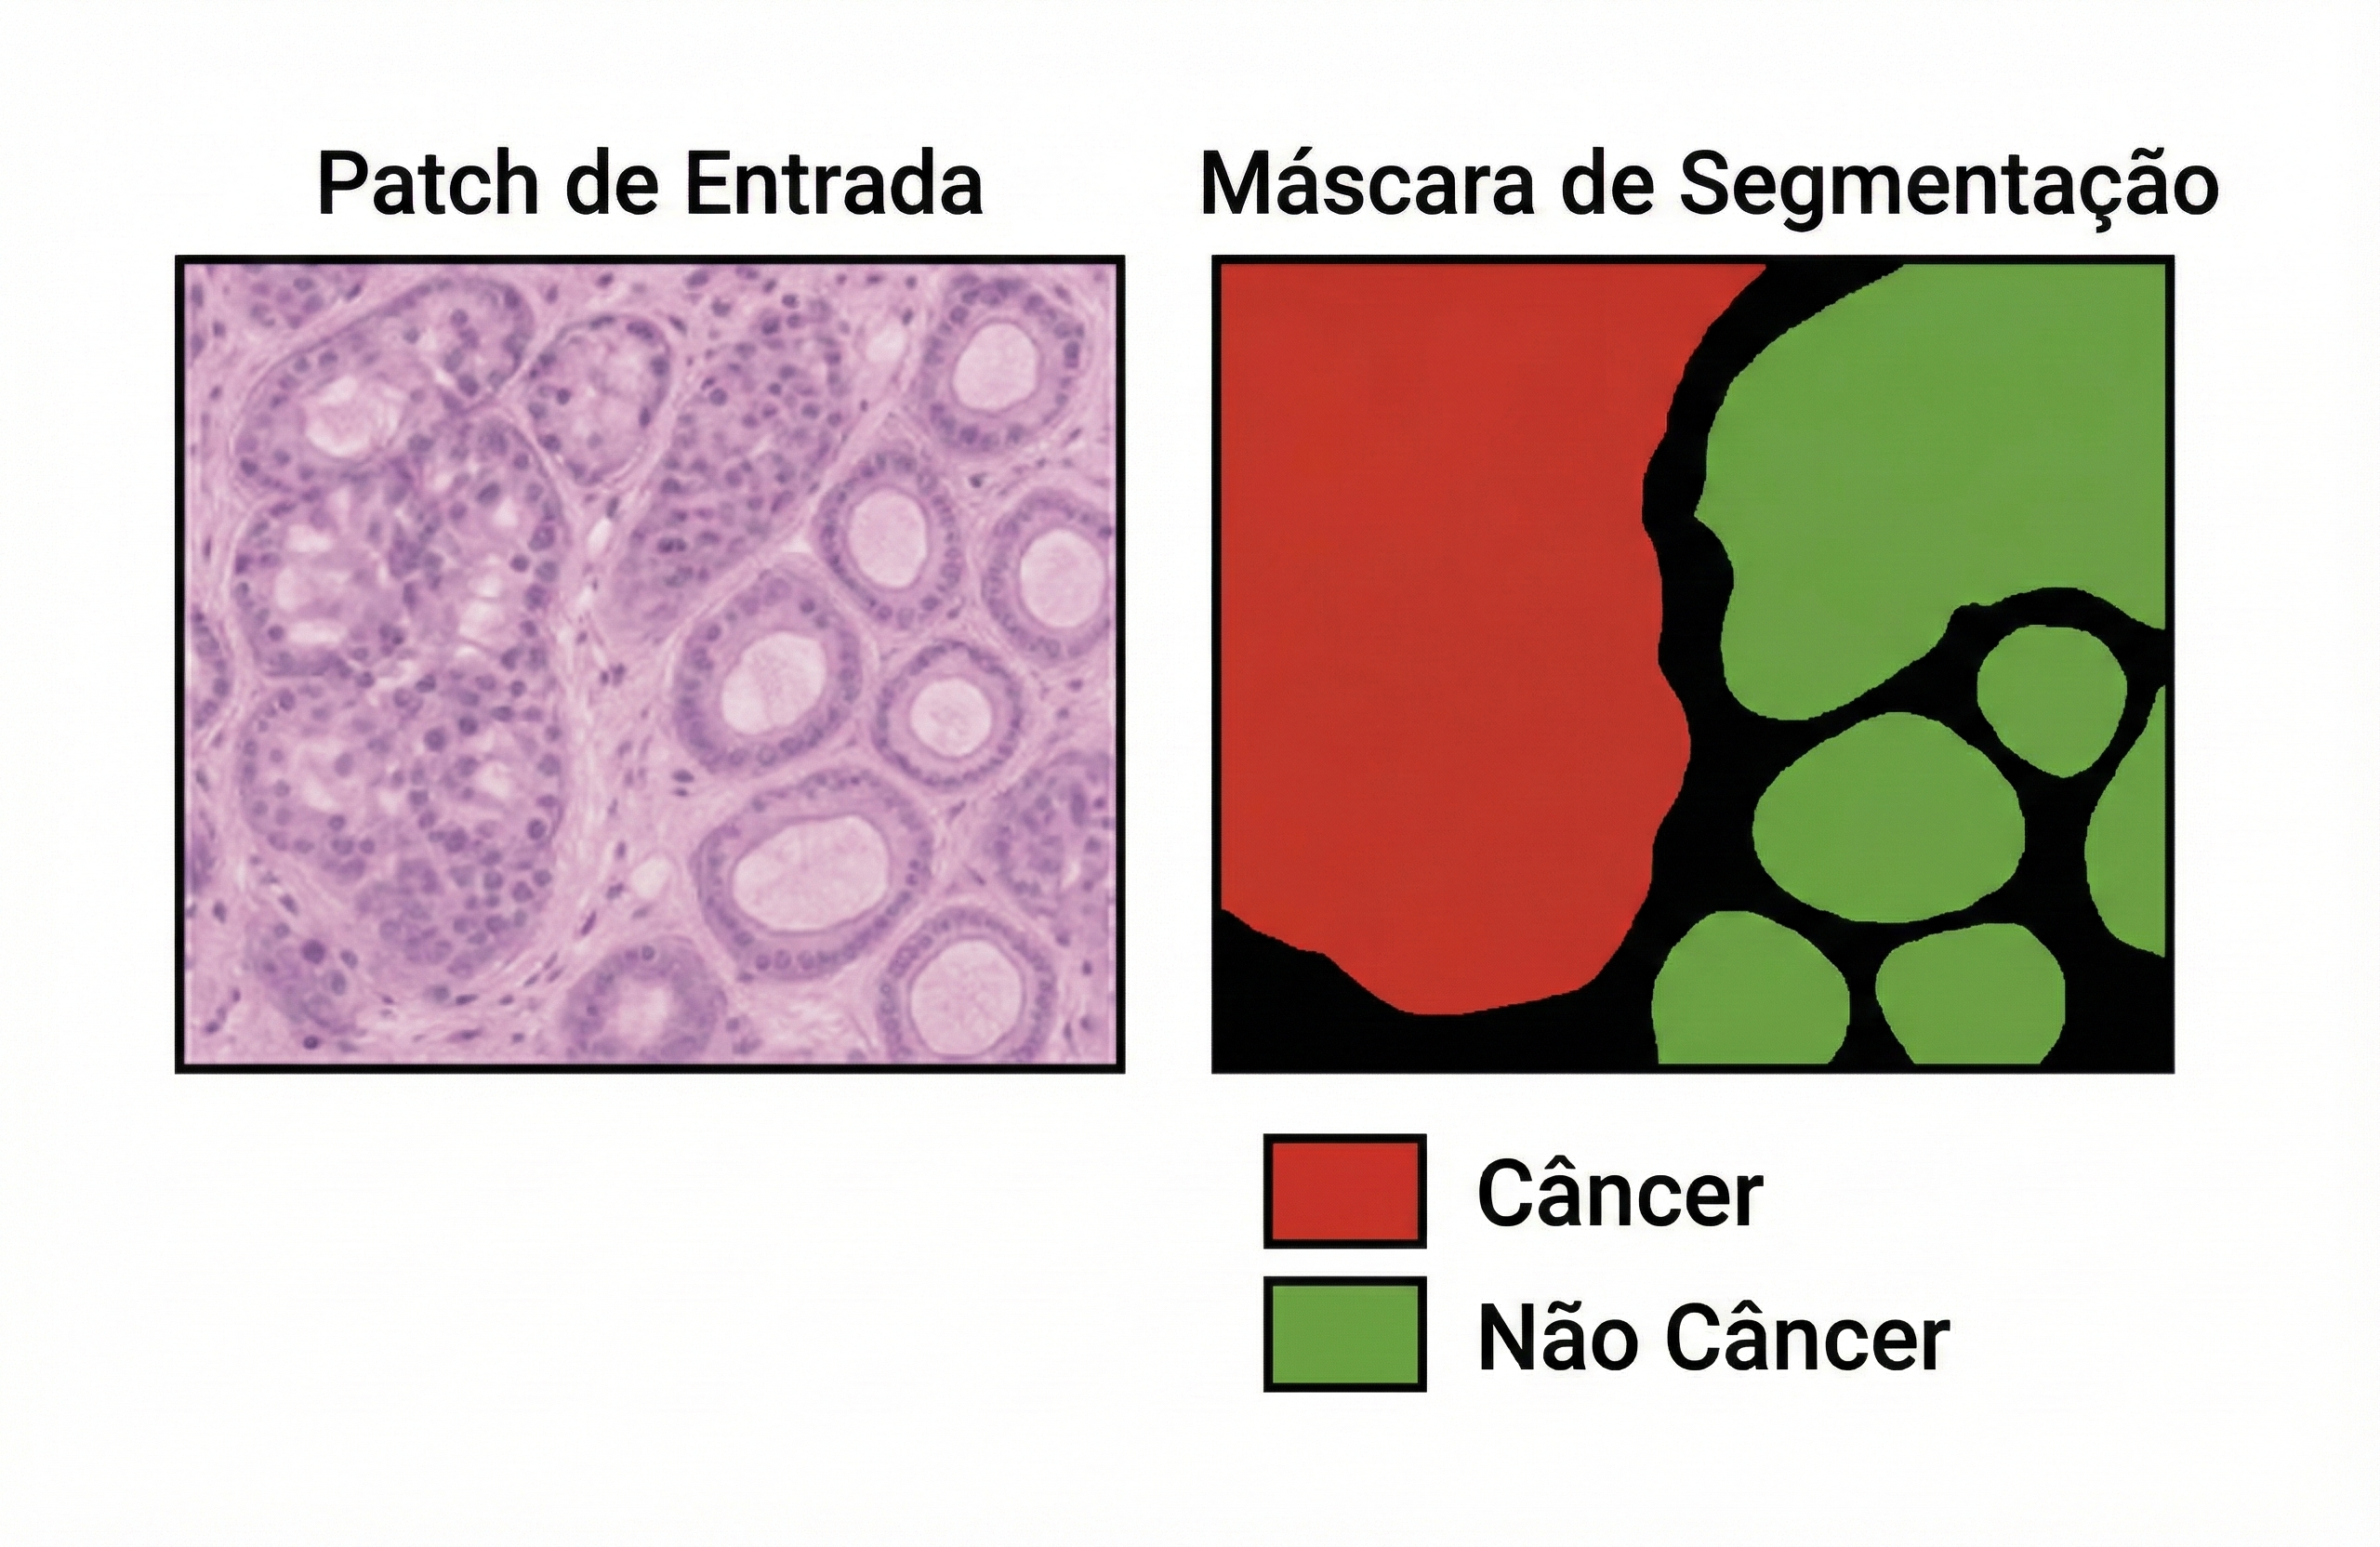
\includegraphics[width=0.82\textwidth]{figuras/semantic_segmentation.png} \caption[Segmentação semântica]{Representação conceitual de segmentação semântica. A imagem de entrada é processada por um modelo que atribui uma classe a cada pixel, produzindo uma máscara de predição espacialmente alinhada à imagem original. Imagem gerada por ferramenta de IA (Gemini).} \label{fig:semantic-segmentation} \end{figure}

\subsection{Redes neurais para segmentação} \label{subsec:redes_segmentacao}

Modelos de segmentação semântica precisam conciliar duas exigências complementares. A primeira é semântica: reconhecer padrões visuais associados às classes de interesse, como regiões tumorais e não tumorais. A segunda é espacial: preservar a localização e o contorno das regiões segmentadas. Por essa razão, muitas arquiteturas de segmentação adotam estruturas do tipo codificador--decodificador. O codificador extrai representações progressivamente mais abstratas da imagem, enquanto o decodificador projeta essas representações de volta para uma grade espacial compatível com a máscara de saída. 

Arquiteturas convolucionais constituem uma das principais famílias empregadas em segmentação semântica. Modelos como U-Net, UNet++, DeepLabv3+, FPN e MA-Net exploram filtros locais, conexões entre diferentes níveis de resolução, fusões multiescala e mecanismos de atenção para reconstruir máscaras densas. Essas estruturas são particularmente adequadas para capturar padrões locais e preservar detalhes espaciais, aspectos relevantes em imagens histológicas, nas quais fronteiras, texturas e arranjos glandulares podem ter importância diagnóstica. 

Em contrapartida, arquiteturas baseadas em \textit{Transformers}, como Swin, DPT, SegFormer e UPerNet, introduzem formas alternativas de modelar contexto. Esses modelos organizam a imagem em unidades de representação, frequentemente tratadas como \textit{tokens}, e utilizam mecanismos de atenção para capturar relações entre regiões. Dependendo da arquitetura, essa modelagem pode ocorrer por atenção em janelas, codificadores hierárquicos, agregação multiescala ou fusão entre representações locais e globais. A \Figura{fig:arquiteturas-conceituais} resume, em nível conceitual, a diferença entre uma rede convolucional e um \textit{Transformer} visual. 

\begin{figure}[!htb] \centering \begin{subfigure}{0.48\textwidth} \centering 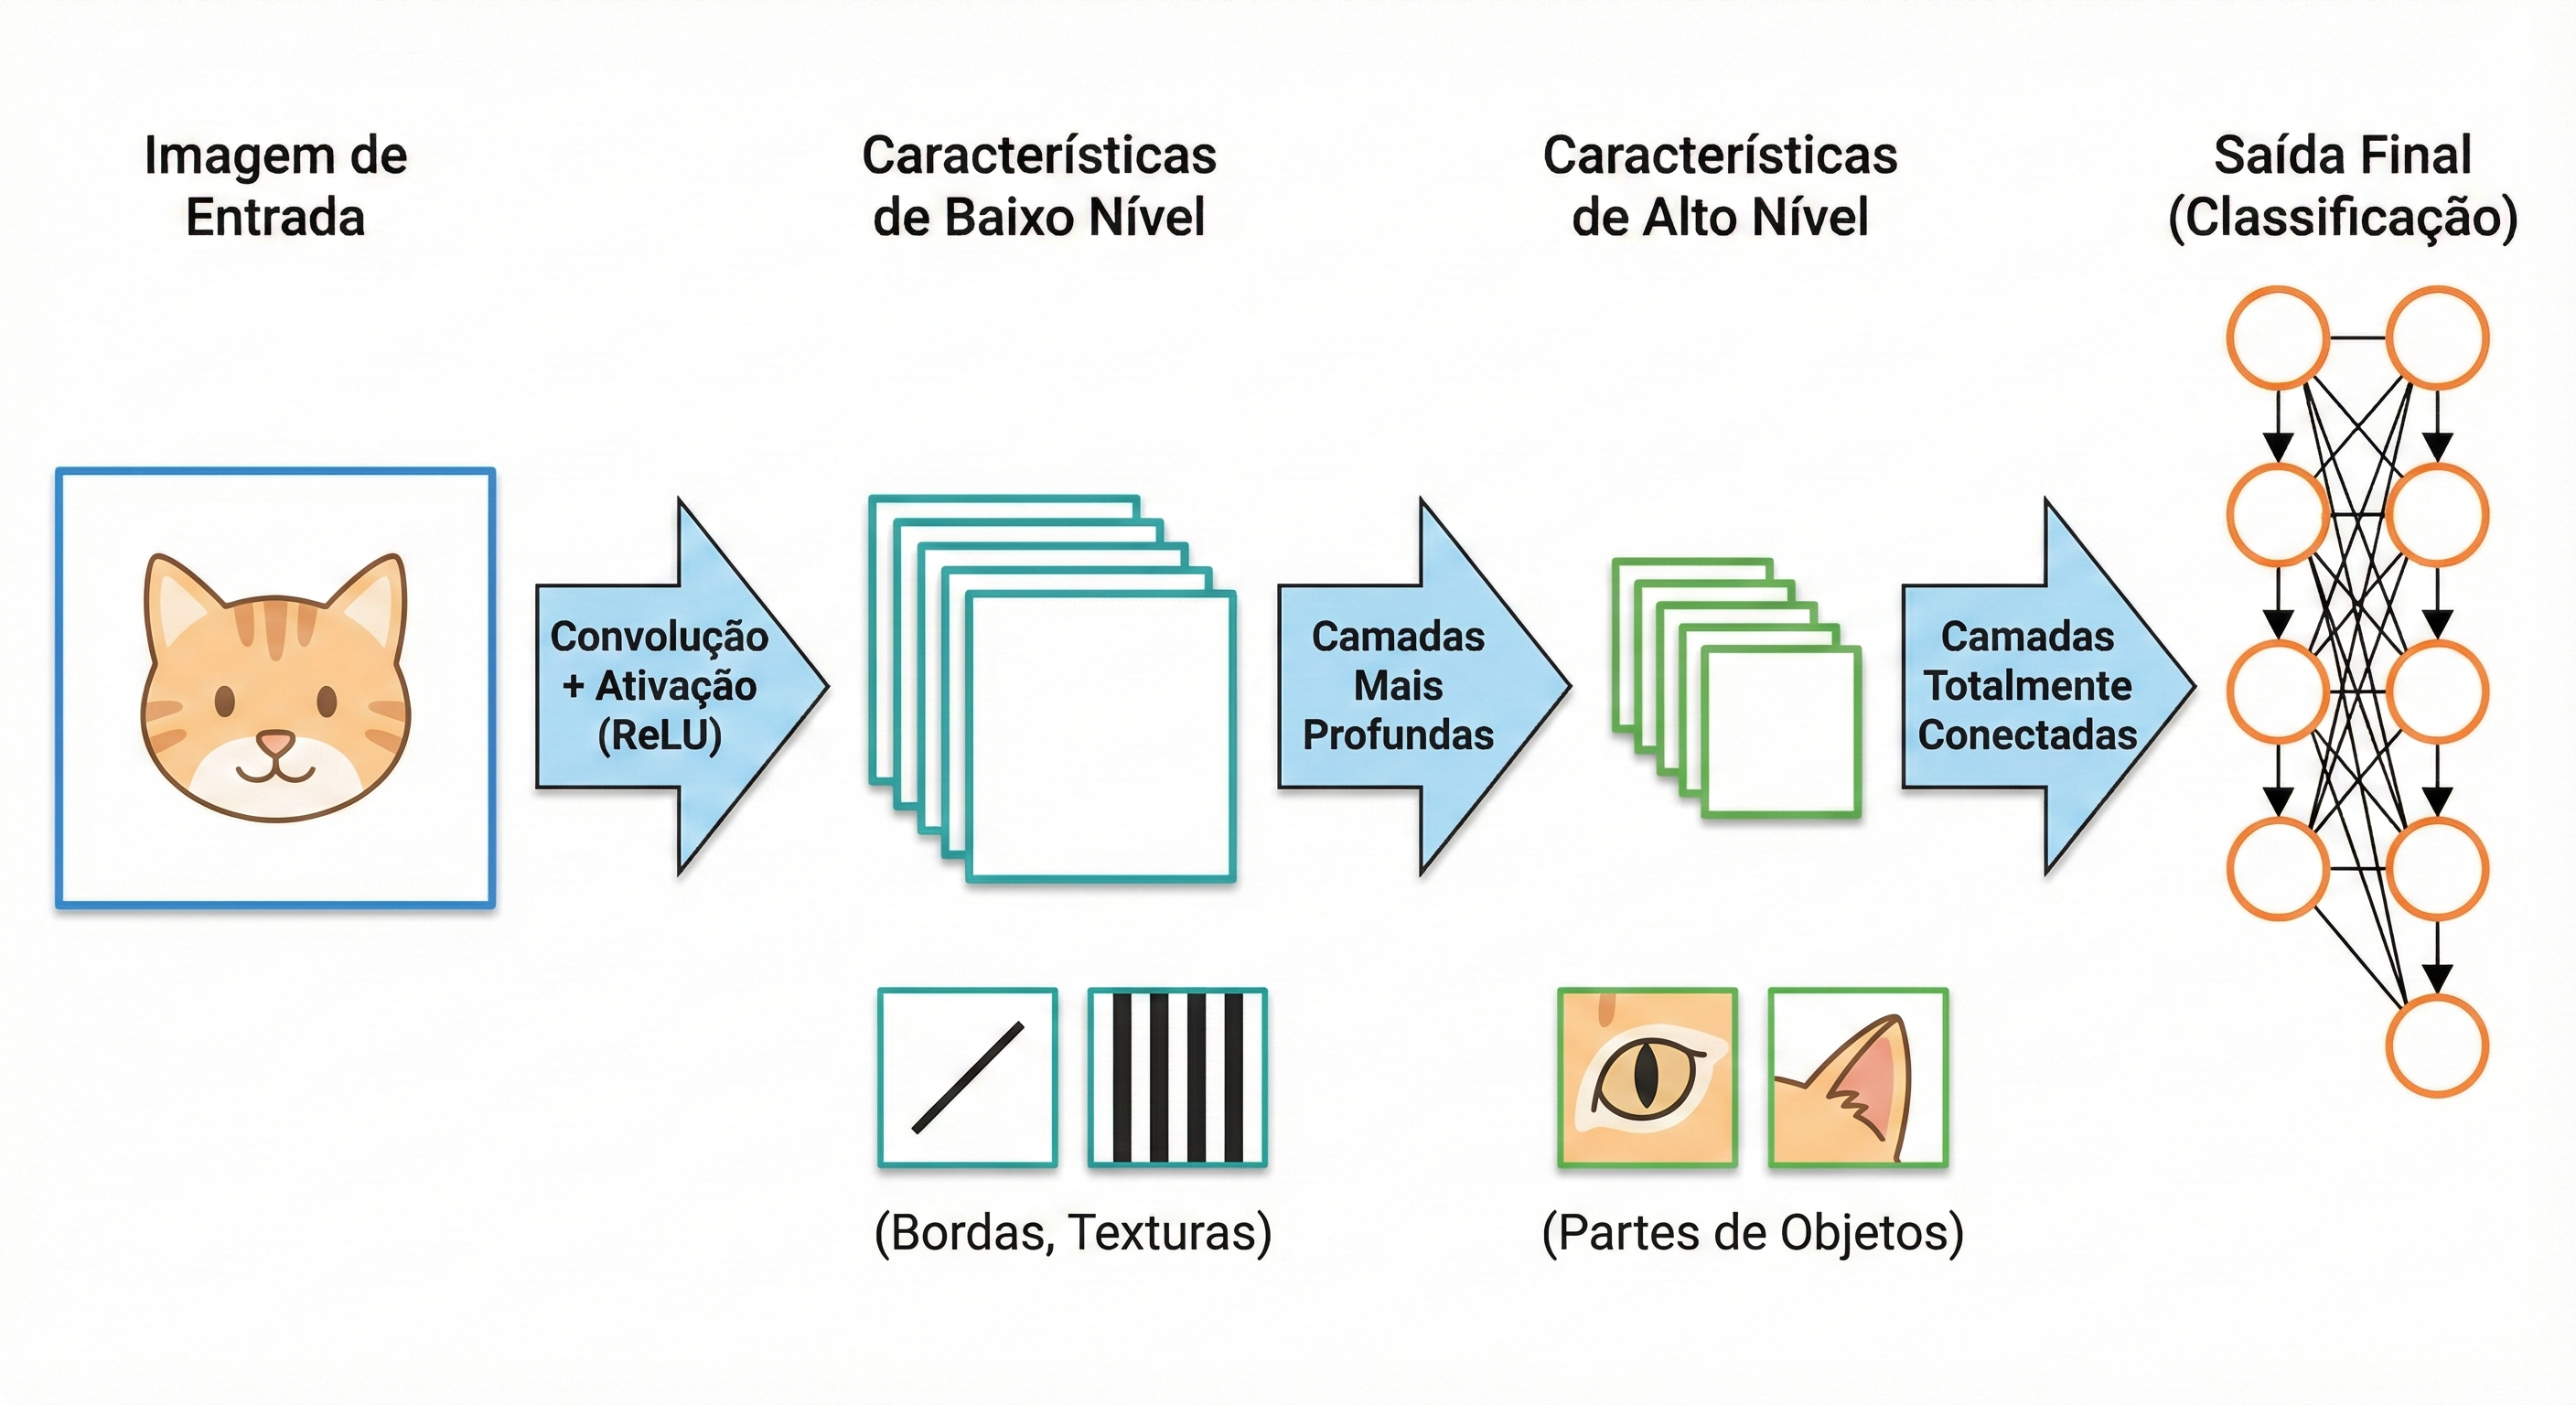
\includegraphics[width=\linewidth]{figuras/CNN.png} \caption{Rede convolucional} \label{fig:cnn-conceito} \end{subfigure}\hfill \begin{subfigure}{0.48\textwidth} \centering 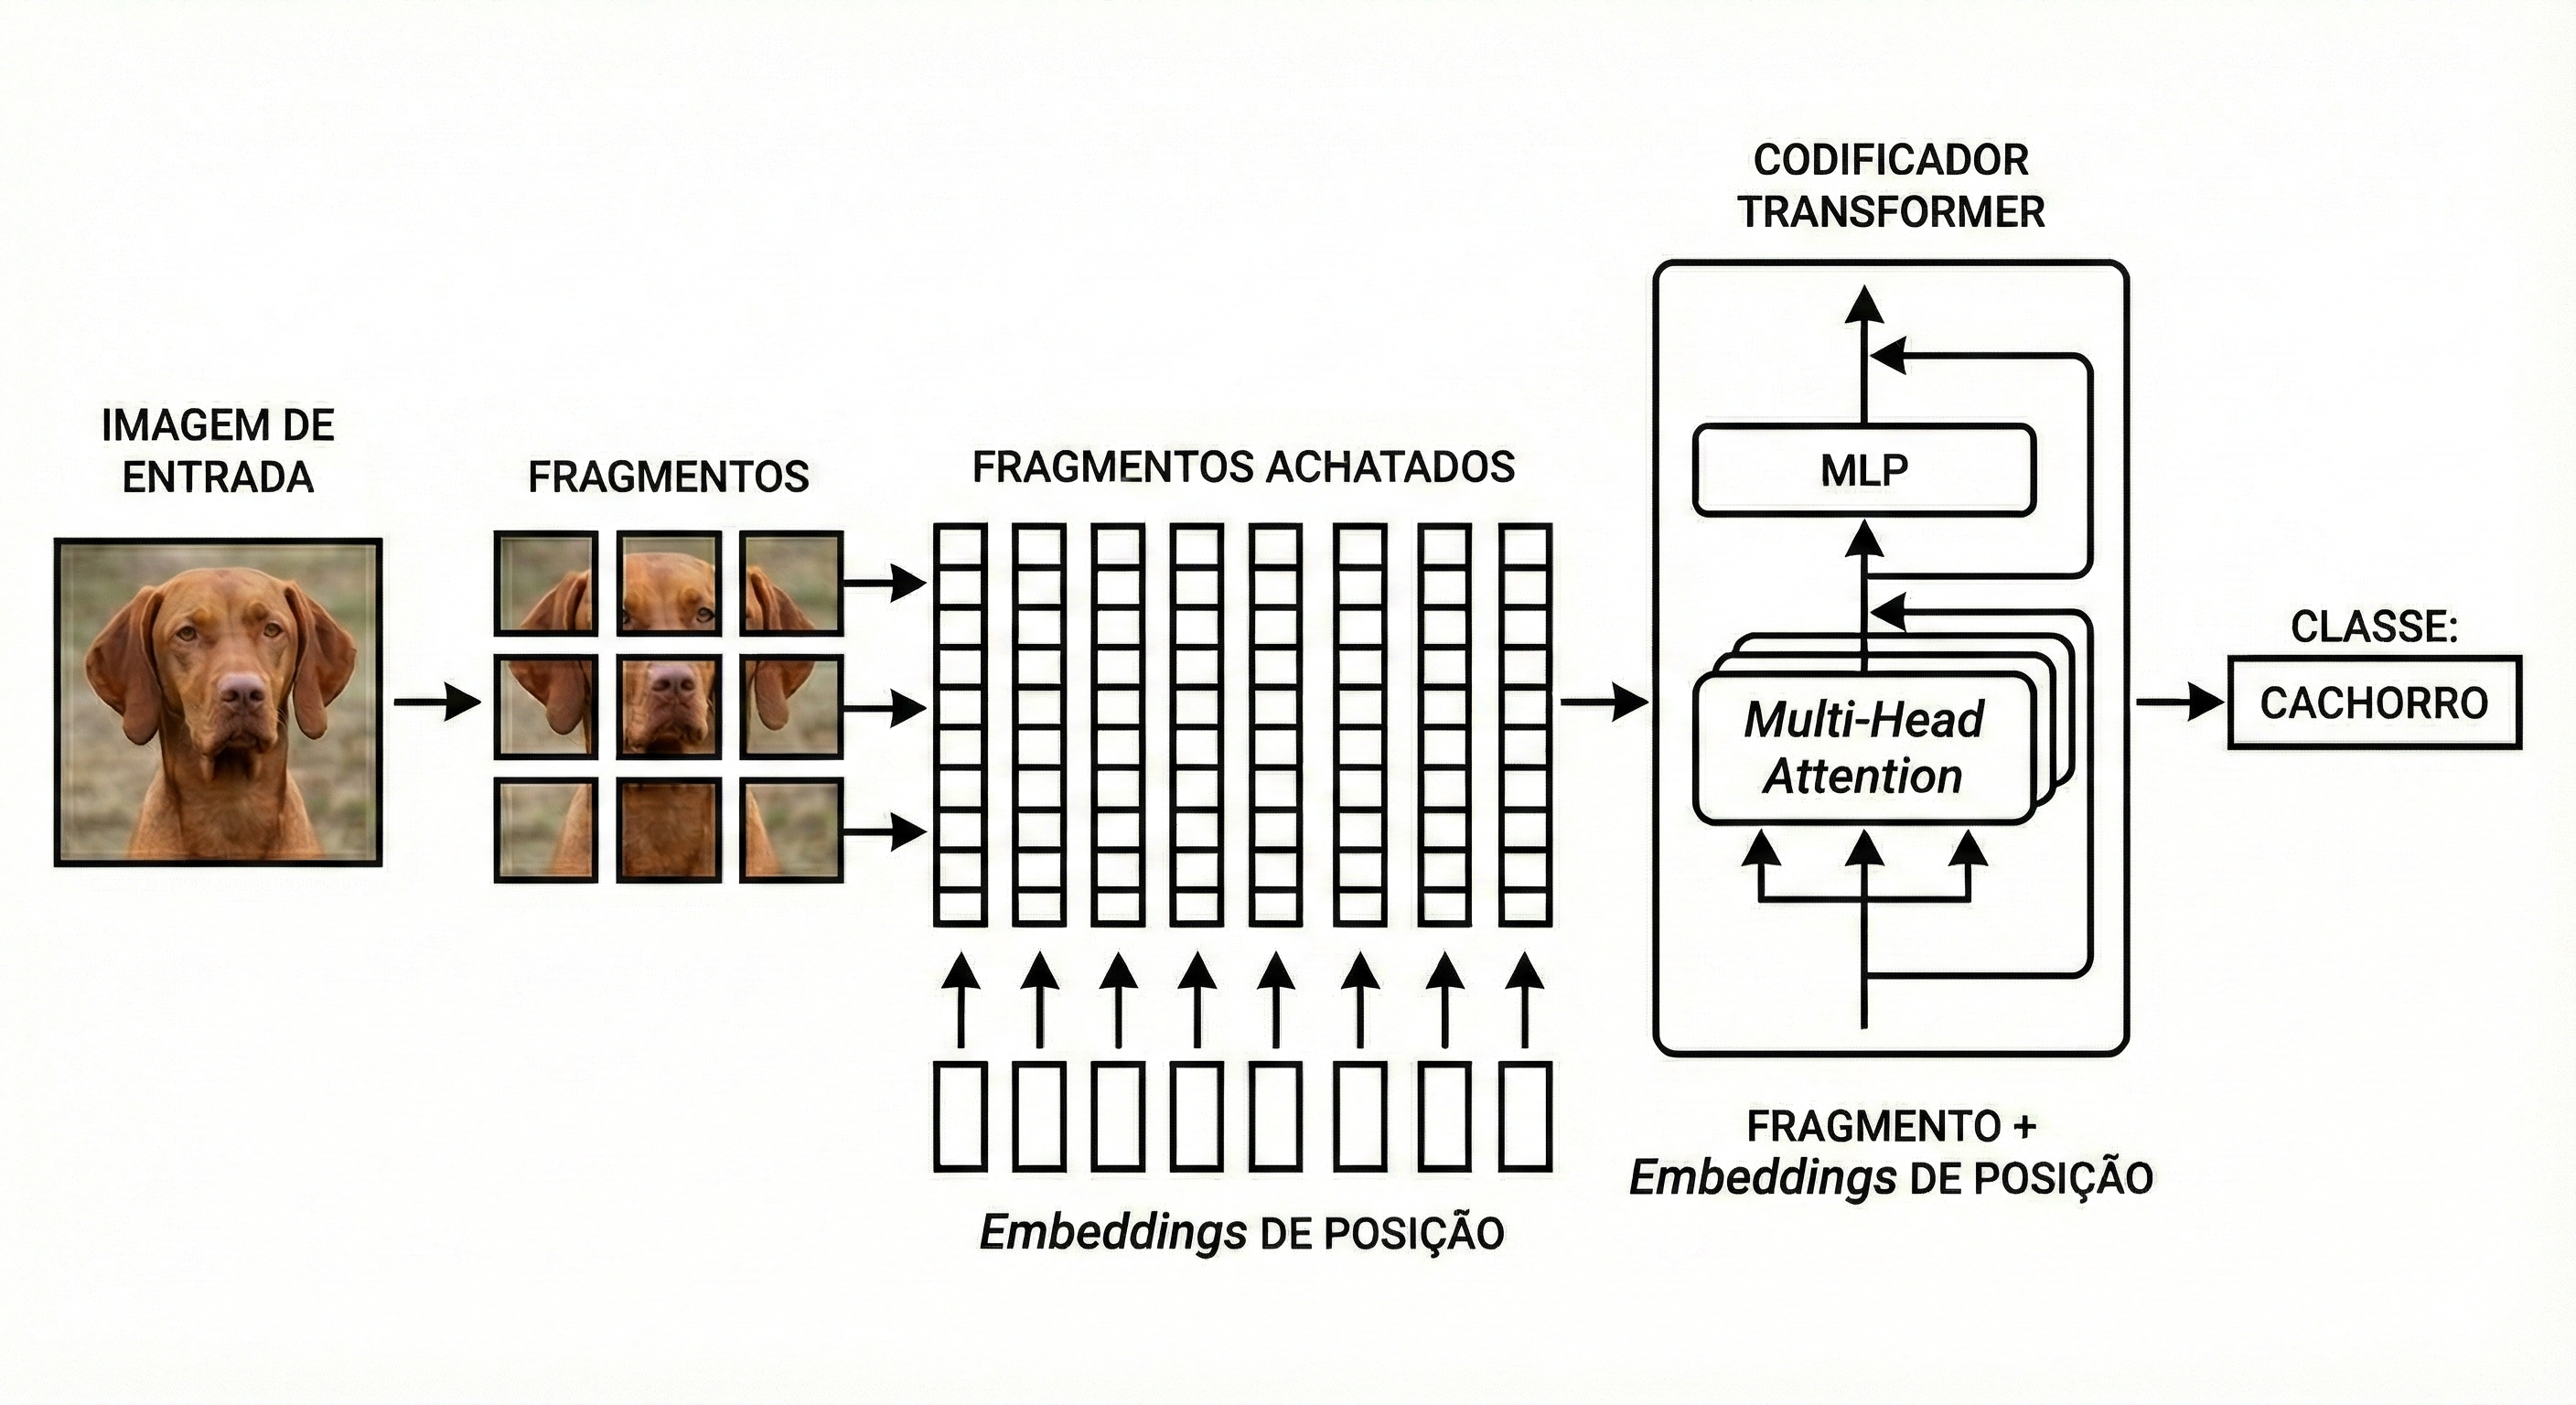
\includegraphics[width=\linewidth]{figuras/vit_architecture.png} \caption{\textit{Transformer} visual} \label{fig:vit-conceito} \end{subfigure} \caption[Arquiteturas neurais em visão computacional]{Representações conceituais de famílias arquiteturais usadas em visão computacional. Redes convolucionais enfatizam a extração local por filtros compartilhados, enquanto \textit{Transformers} visuais organizam a imagem em unidades de representação e usam mecanismos de atenção para modelar relações entre regiões. Imagem gerada por ferramenta de IA (Gemini).} \label{fig:arquiteturas-conceituais} \end{figure}


\subsection{Pré-treinamento em \textit{ImageNet}} \label{subsec:pretreinamento_imagenet} 

Em tarefas de segmentação, arquiteturas neurais frequentemente utilizam \textit{encoders} inicializados com pesos pré-treinados em grandes bases de imagens, como a \textit{ImageNet}, antes do ajuste ao domínio específico de aplicação. Essa estratégia constitui uma forma de transferência de aprendizado: em vez de iniciar todos os parâmetros de maneira aleatória, o modelo parte de representações visuais previamente aprendidas em uma base ampla de imagens naturais. 

Embora imagens naturais e imagens histopatológicas pertençam a domínios distintos, o pré-treinamento pode oferecer uma inicialização útil para a extração de padrões visuais genéricos, como bordas, texturas, contrastes locais e composições estruturais. Com isso, tende a reduzir a dependência de grandes volumes de dados anotados no domínio-alvo e a favorecer uma trajetória de otimização mais estável durante o treinamento. 

O \textit{ImageNet} é uma base de imagens em larga escala amplamente utilizada em visão computacional, sobretudo em tarefas de reconhecimento visual \cite{deng2009imagenet,russakovsky2015imagenet}. Por sua abrangência, escala e impacto histórico, tornou-se uma referência importante para treinamento, avaliação e pré-treinamento de modelos de aprendizagem profunda. 

\begin{figure}[!htb] \centering 
\includegraphics[width=\linewidth]{figuras/imagenet.png} \caption[\textit{ImageNet} como base de pré-treinamento]{\textit{ImageNet}, grande base de dados composta por 14.197.122 imagens e 21.841 \textit{synsets} indexados. Cada \textit{synset} corresponde a um conceito semântico definido, ao qual são associadas imagens anotadas e submetidas a controle de qualidade. Essa estrutura tornou o \textit{ImageNet} uma referência para treinamento, avaliação e pré-treinamento de modelos de reconhecimento visual.} \label{fig:imagenet-conceito} \end{figure}

\subsection{Arquiteturas convolucionais} \label{subsec:arquiteturas_convolucionais} 

Redes convolucionais permanecem relevantes em segmentação biomédica porque combinam eficiência computacional, viés indutivo local e capacidade de recuperar detalhes espaciais. Em histopatologia, esses aspectos são importantes para representar textura, bordas glandulares, transições entre tecido tumoral e não tumoral e pequenos padrões morfológicos distribuídos no \textit{patch}. 

A \Tabela{tab:cnn-models} resume arquiteturas convolucionais frequentemente empregadas em tarefas de segmentação semântica. A tabela distingue o princípio arquitetural de cada família e sua respectiva referência, com ênfase em mecanismos relevantes para reconstrução espacial, fusão multiescala e preservação de detalhes locais. 

\begin{table}[!htb] \centering \caption{Arquiteturas convolucionais consideradas na fundamentação teórica.} \label{tab:cnn-models} \begin{tabular}{p{2.8cm}p{8.4cm}p{3.0cm}} \toprule Arquitetura & Princípio arquitetural & Referência \\ \midrule DeepLabv3+ & Arquitetura codificador--decodificador que combina convoluções, agregação de contexto multiescala e refinamento espacial da predição. & \cite{chen2018deeplabv3plus} \\ UNet++ & Extensão da U-Net com conexões densas e aninhadas entre codificador e decodificador, proposta para reduzir a lacuna semântica entre mapas de características de diferentes níveis. & \cite{zhou2020unetpp} \\ FPN & Rede de pirâmide de características que combina mapas de alta resolução com representações semanticamente mais abstratas, favorecendo predições multiescala. & \cite{lin2017fpn} \\ MA-Net & Arquitetura baseada em U-Net que incorpora mecanismos de atenção multiescala para integrar informações locais e globais durante a reconstrução da máscara. & \cite{fan2020manet} \\ \bottomrule \end{tabular} \end{table} 

Essas arquiteturas ilustram diferentes formas de explorar o viés convolucional em segmentação densa. Embora também capturem informação semântica, sua estrutura favorece a reconstrução local, a integração de mapas em múltiplas resoluções e a preservação de detalhes espaciais. Por isso, permanecem especialmente relevantes em imagens histológicas, nas quais pequenas variações de textura, contorno e organização tecidual podem influenciar a delimitação das regiões de interesse.

\subsection{Arquiteturas baseadas em \textit{Transformers}} \label{subsec:arquiteturas_transformers} 

\textit{Transformers} visuais adaptam mecanismos de atenção para o processamento de imagens. Em vez de depender exclusivamente de filtros convolucionais locais, essas arquiteturas representam a imagem por unidades ou regiões e calculam relações entre elas por meio de atenção. O mecanismo de atenção escalada por produto interno pode ser resumido por: 

\begin{equation}\label{eq:attention} \mathrm{Attention}(Q,K,V)= \mathrm{softmax}\left(\frac{QK^\top}{\sqrt{d_k}}\right)V, \end{equation} em que $Q$, $K$ e $V$ são matrizes de consulta, chave e valor, respectivamente, e $d_k$ é a dimensão das chaves \cite{dosovitskiy2021vit}. 

Em WSIs, esse tipo de mecanismo é relevante porque permite representar relações mais amplas do que aquelas capturadas por filtros estritamente locais. Essa capacidade pode auxiliar a integração de contexto entre regiões do tecido, especialmente em tarefas nas quais a interpretação local depende de padrões distribuídos em diferentes áreas da imagem. Em contrapartida, o custo computacional da atenção precisa ser controlado, sobretudo quando se trabalha com \textit{patches} de alta resolução ou grandes volumes de amostras. Por isso, arquiteturas modernas adotam estratégias como atenção em janelas, codificadores hierárquicos, agregação multiescala e decodificadores leves. 

A \Tabela{tab:transformer-models} resume arquiteturas baseadas em \textit{Transformers} relevantes para tarefas de predição densa em visão computacional. 

\begin{table}[!htb] \centering \caption{Arquiteturas baseadas em \textit{Transformers} consideradas na fundamentação teórica.} \label{tab:transformer-models} \begin{tabular}{p{2.8cm}p{8.4cm}p{3.0cm}} \toprule Arquitetura & Princípio arquitetural & Referência \\ \midrule Swin & \textit{Transformer} hierárquico com atenção em janelas deslocadas, projetado para reduzir custo computacional e preservar representações multiescala. & \cite{liu2021swin} \\ DPT & Arquitetura de predição densa que combina representações intermediárias de um \textit{Vision Transformer} e as projeta para uma saída espacial. & \cite{ranftl2021dpt} \\ SegFormer & Estrutura de segmentação que combina codificador \textit{Transformer} hierárquico com decodificador \Sigla{\textit{multi-layer perceptron}}{MLP} leve para agregação multiescala. & \cite{xie2021segformer} \\ UPerNet & Estrutura de segmentação multiescala proposta para \textit{unified perceptual parsing}, utilizada para integrar representações hierárquicas em predições densas. & \cite{xiao2018upernet} \\ \bottomrule \end{tabular} \end{table} 

Essas arquiteturas ilustram diferentes estratégias para incorporar contexto em predições densas. Enquanto algumas reduzem o custo da atenção por meio de janelas locais, outras combinam representações hierárquicas e fusão multiescala para recuperar uma saída espacialmente organizada. Desse modo, modelos baseados em \textit{Transformers} ampliam o conjunto de vieses arquiteturais disponíveis para segmentação semântica, complementando abordagens convolucionais na representação de padrões locais e contextuais.

\section{Métricas de avaliação}\label{sec:metricas_reprodutibilidade} 

A avaliação de modelos de segmentação em patologia digital deve considerar tanto a qualidade espacial das máscaras preditas quanto a capacidade discriminativa das probabilidades produzidas pelo modelo. Métricas como o Coeficiente de Dice, o Coeficiente de Correlação de Matthews (\Sigla{\textit{Matthews Correlation Coefficient}}{MCC}), a área sob a curva ROC (\Sigla{\textit{Area Under the Receiver Operating Characteristic Curve}}{AUROC}) e a área sob a curva precisão-revocação (\Sigla{\textit{Area Under the Precision-Recall Curve}}{AUPRC}) são complementares, pois capturam aspectos distintos do desempenho: sobreposição espacial, correlação entre predição e referência, discriminação probabilística e comportamento sob desbalanceamento. 

Para obter uma máscara binária a partir da probabilidade predita pelo modelo, é necessário definir um limiar de decisão. Seja $p_i$ a probabilidade atribuída ao pixel $i$ de pertencer à classe positiva. A predição binária $\hat{y}_i(t)$ para um limiar $t$ pode ser escrita como: 

\begin{equation}\label{eq:threshold-prediction} \hat{y}_i(t) = \begin{cases} 1, & \text{se } p_i \geq t,\\ 0, & \text{se } p_i < t. \end{cases} \end{equation} 

A partir da comparação entre $\hat{y}_i(t)$ e a máscara de referência $y_i$, obtêm-se as quantidades da matriz de confusão em nível de pixel: \Sigla{\textit{Verdadeiros Positivos}}{TP}, \Sigla{\textit{Falsos Positivos}}{FP}, \Sigla{\textit{Verdadeiros Negativos}}{TN} e \Sigla{\textit{Falsos Negativos}}{FN}. Métricas como Dice e MCC dependem dessas contagens e, portanto, também dependem do limiar escolhido. 

O Coeficiente de Dice mede a sobreposição entre a região positiva prevista e a região positiva de referência: 

\begin{equation}\label{eq:dice-revisao} \mathrm{Dice} = \frac{2TP}{2TP+FP+FN}. \end{equation} 

Em segmentação, essa métrica é intuitiva porque avalia diretamente a concordância espacial entre máscara prevista e máscara anotada. Entretanto, comparações baseadas em Dice devem explicitar a unidade de agregação, o tratamento de máscaras vazias e o limiar usado para binarizar as probabilidades \cite{seghier2024dice}.

O MCC resume a associação entre predição binária e referência considerando, em uma única expressão, os quatro termos da matriz de confusão:

\begin{equation}\label{eq:mcc} \mathrm{MCC} = \frac{TP \cdot TN - FP \cdot FN} {\sqrt{(TP+FP)(TP+FN)(TN+FP)(TN+FN)}}. \end{equation} 

Seu valor varia de $-1$ a $1$: valores próximos de $1$ indicam forte concordância entre predição e referência; valores próximos de $0$ indicam desempenho próximo ao acaso; e valores negativos indicam discordância sistemática. Em cenários desbalanceados, o MCC é particularmente útil porque penaliza simultaneamente erros na classe positiva e na classe negativa, evitando interpretações excessivamente otimistas baseadas apenas em acurácia \cite{chicco2020advantages}.

Além das métricas dependentes de limiar, existem métricas independentes de limiar, calculadas a partir da variação do ponto de decisão sobre as probabilidades preditas. A curva ROC relaciona a sensibilidade (\Sigla{\textit{True Positive Rate}}{TPR}) e a taxa de falsos positivos (\Sigla{\textit{False Positive Rate}}{FPR}) para diferentes valores de $t$: \begin{equation}\label{eq:tpr-fpr} \mathrm{TPR}(t)=\frac{TP(t)}{TP(t)+FN(t)}, \qquad \mathrm{FPR}(t)=\frac{FP(t)}{FP(t)+TN(t)}. \end{equation} 

A AUROC corresponde à área sob essa curva e avalia a capacidade do modelo de atribuir escores mais altos aos pixels positivos do que aos negativos ao longo dos limiares considerados \cite{fawcett2006roc}. A curva precisão-revocação, por sua vez, relaciona precisão e revocação: 
\begin{equation}\label{eq:precision-recall} \mathrm{Precis\tilde{a}o}(t)=\frac{TP(t)}{TP(t)+FP(t)}, \qquad \text{Revoca\c{c}\~ao}(t)=\frac{TP(t)}{TP(t)+FN(t)}. \end{equation} 

A AUPRC corresponde à área sob essa curva. Em tarefas com forte desbalanceamento, como segmentação de câncer em que a região positiva pode ocupar pequena fração da imagem, a AUPRC tende a ser mais sensível à qualidade das predições positivas do que a AUROC, pois considera diretamente a relação entre falsos positivos e verdadeiros positivos \cite{saito2015precision}. 

A \Figura{fig:roc-conceitual} ilustra a leitura conceitual da curva ROC, enquanto a \Figura{fig:prc-conceitual} apresenta a curva precisão-revocação. Essas curvas complementam as métricas calculadas em um limiar específico: AUROC e AUPRC avaliam o comportamento probabilístico do modelo ao longo de diferentes limiares, enquanto Dice e MCC caracterizam o desempenho após a escolha de um ponto de decisão. 

\begin{figure}[!htb] \centering 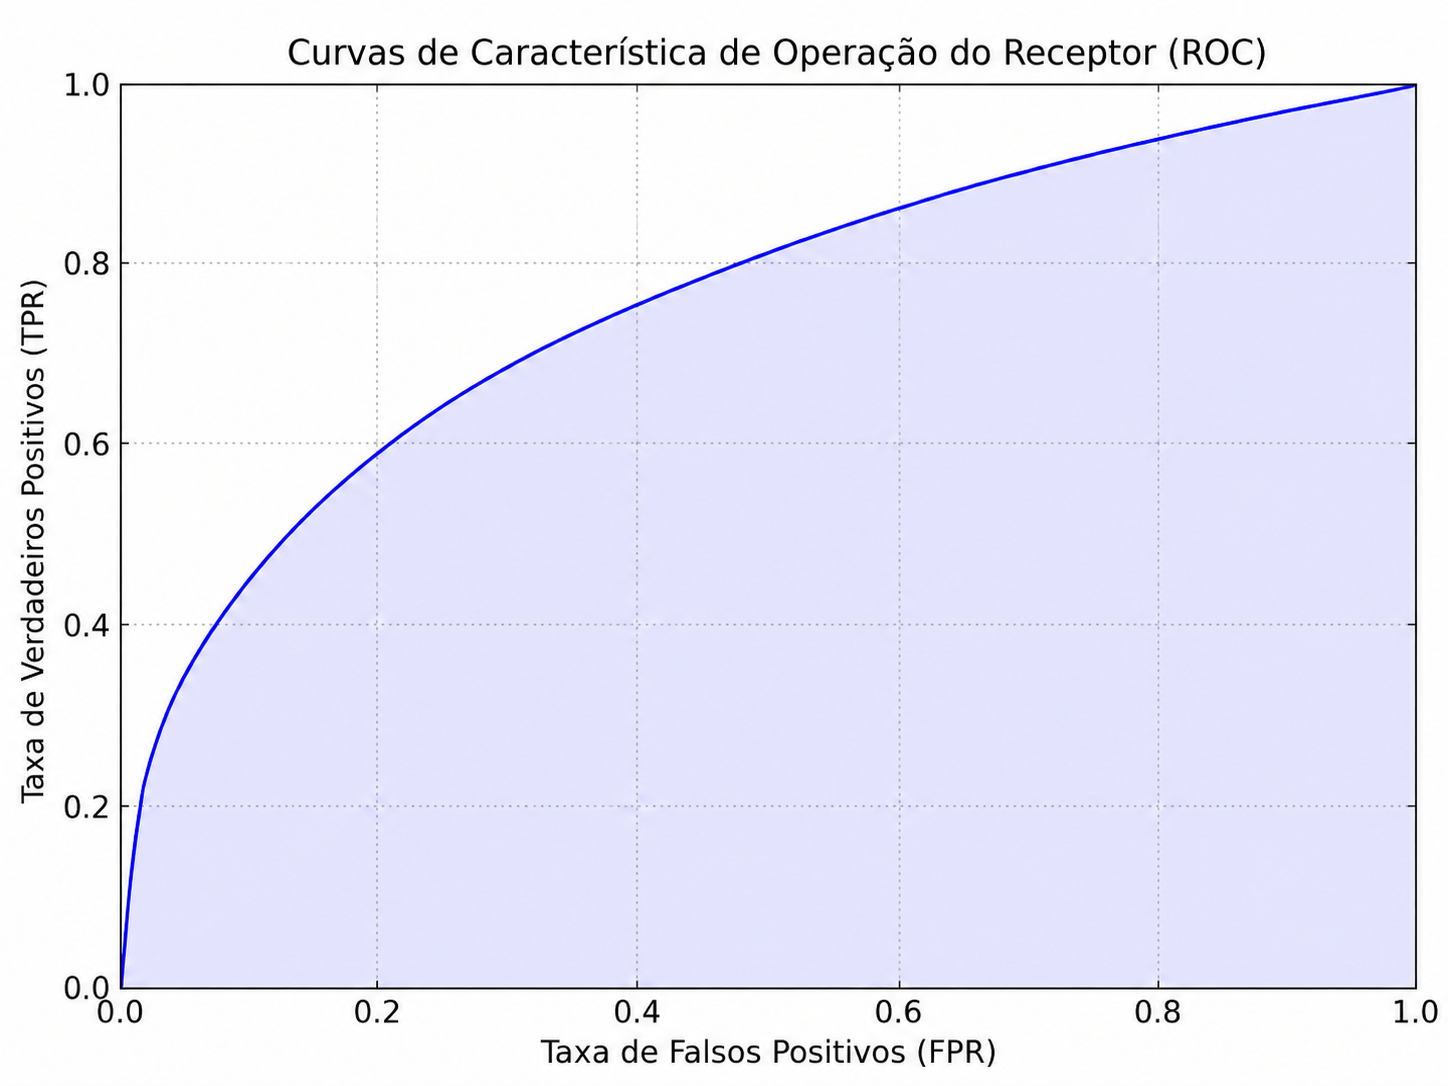
\includegraphics[width=0.68\textwidth]{figuras/roc_curve.png} \caption[Curva ROC conceitual]{Representação conceitual de uma curva ROC. O eixo horizontal indica a taxa de falsos positivos (\textit{false positive rate}, FPR), enquanto o eixo vertical indica a taxa de verdadeiros positivos (\textit{true positive rate}, TPR), também interpretada como sensibilidade. A curva azul ilustra o comportamento do classificador ao longo de diferentes limiares de decisão: quanto mais a curva se aproxima do canto superior esquerdo, maior tende a ser a capacidade discriminativa do modelo. A região sombreada sob a curva representa a área sob a curva ROC (AUROC), utilizada como medida agregada de separação entre as classes ao longo de todos os limiares. Imagem gerada por ferramenta de IA (Gemini).} \label{fig:roc-conceitual} \end{figure} 

\begin{figure}[!htb] \centering 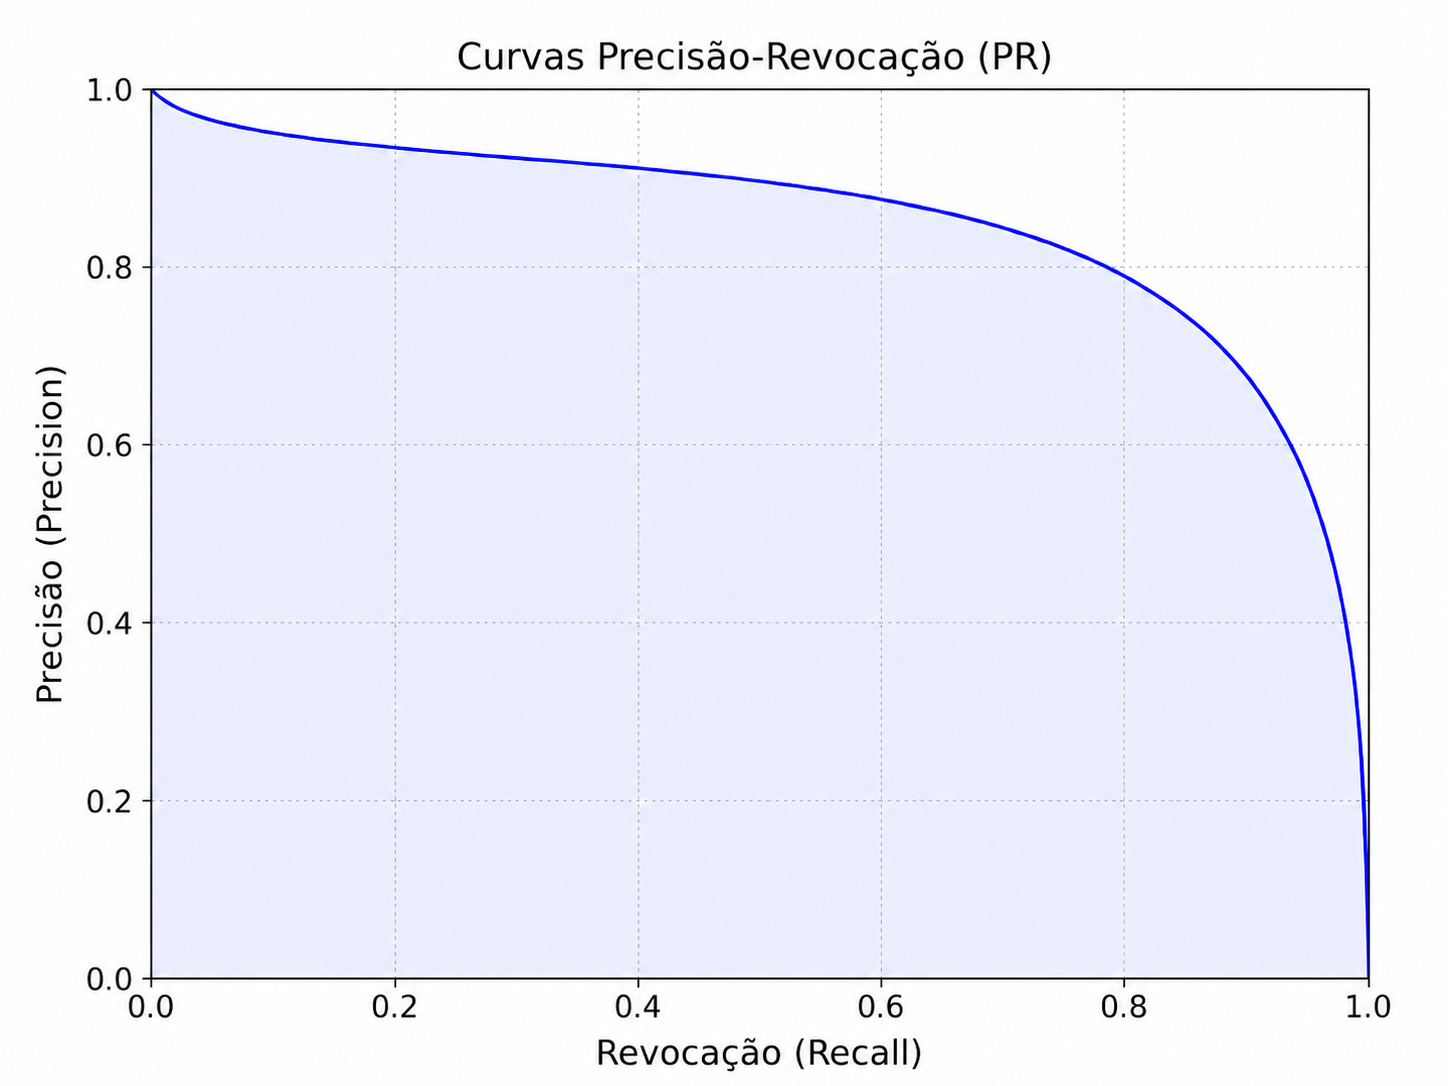
\includegraphics[width=0.68\textwidth]{figuras/auprc_curve.png} \caption[Curva precisão-revocação conceitual]{ Representação conceitual de uma curva precisão-revocação. O eixo horizontal indica a revocação, isto é, a proporção de exemplos positivos corretamente recuperados, enquanto o eixo vertical indica a precisão, isto é, a proporção de predições positivas que correspondem à classe positiva. A curva azul representa o desempenho do modelo ao longo de diferentes limiares de decisão, e a região sombreada sob essa curva corresponde à área sob a curva precisão-revocação, ou AUPRC. Em tarefas desbalanceadas, como a segmentação de regiões tumorais, essa visualização é particularmente informativa por evidenciar o compromisso entre recuperar a classe positiva e controlar a quantidade de falsos positivos. Imagem gerada por ferramenta de IA (Gemini).} \label{fig:prc-conceitual} \end{figure}

\section{Reprodutibilidade e auditoria} \label{sec:reprodutibilidade_ferramentas}

Em dados médicos, múltiplas amostras podem derivar da mesma lâmina, do mesmo caso ou do mesmo paciente. Em fluxos baseados em \textit{patches}, essa dependência é especialmente crítica: recortes visualmente semelhantes podem aparecer em diferentes conjuntos experimentais quando o particionamento é feito em nível de amostra. Nessa situação, o modelo pode ser avaliado sobre padrões muito próximos daqueles observados durante o treinamento, produzindo uma estimativa artificialmente otimista de desempenho. Por essa razão, a separação por identificador de paciente e a validação agrupada constituem princípios metodológicos centrais em experimentos de aprendizagem profunda com dados médicos \cite{roberts2017crossvalidation,dawood2026confounding}. 

A reprodutibilidade também depende da preservação dos artefatos que conectam dados, decisões experimentais e resultados. Manifestos, assinaturas de arquivos, configurações, relatórios, \textit{checkpoints}, métricas e \textit{logs} permitem reconstruir o caminho entre os dados de origem, as amostras derivadas, os modelos treinados e as predições avaliadas. Sem esses registros, a métrica reportada torna-se difícil de auditar, pois não é possível determinar com precisão quais dados foram usados, quais transformações foram aplicadas, quais versões de configuração foram executadas e quais artefatos deram origem ao resultado final. 

Essa preocupação se alinha aos princípios FAIR, que enfatizam a necessidade de tornar dados e metadados localizáveis, acessíveis, interoperáveis e reutilizáveis \cite{wilkinson2016fair}. Também é coerente com recomendações de reprodutibilidade computacional, segundo as quais os passos de uma análise devem ser descritos com detalhe suficiente para permitir verificação, reconstrução e comparação por outros pesquisadores \cite{piccolo2016tools}.

\section{\textit{Ensembles}} \label{sec:ensembles_revisao} 

\textit{Ensembles} consistem na combinação de múltiplos modelos com o objetivo de produzir predições mais robustas do que aquelas obtidas por um único modelo isolado. Em tarefas de segmentação, essa combinação pode explorar a complementaridade entre modelos que capturam diferentes aspectos da imagem, como textura, contorno, contexto local e relações espaciais mais amplas. Assim, em vez de tratar todas as predições como equivalentes, a composição pode ser organizada de modo a combinar modelos com vieses arquiteturais distintos \cite{caruana2004ensemble}. 

Essa estratégia é particularmente relevante em patologia digital, pois WSIs combinam informação microscópica local e contexto tecidual em múltiplas escalas. Padrões como textura, arquitetura glandular, transições entre tecido tumoral e não tumoral e distribuição espacial das regiões anotadas podem ser representados de maneira distinta por arquiteturas convolucionais e modelos baseados em \textit{Transformers}. Nesse cenário, \textit{ensembles} oferecem uma forma de integrar predições complementares, reduzindo a dependência de uma única hipótese arquitetural. 

Do ponto de vista metodológico, a composição de um \textit{ensemble} deve ser definida a partir de critérios estabelecidos no conjunto de validação e mantida fixa durante a avaliação final. Esse cuidado reduz o risco de ajuste indireto ao conjunto de teste e preserva a separação entre seleção de modelos e estimação de desempenho. Portanto, além de melhorar a robustez preditiva, \textit{ensembles} também exigem documentação explícita dos modelos combinados, dos pesos ou regras de agregação e do critério utilizado para definir a configuração final.

\section{Revisão estruturada da literatura recente} \label{sec:revisao_literatura_recente} 

Esta seção apresenta uma revisão bibliográfica estruturada da literatura recente sobre fluxos de patologia digital oncológica baseados em aprendizagem profunda. A revisão complementa a fundamentação conceitual do capítulo ao examinar, nos artigos selecionados por critérios previamente definidos de busca e elegibilidade, como são descritas decisões que afetam a validade experimental: controle de qualidade e tratamento de artefatos, prevenção de vazamento de dados, governança e rastreabilidade dos dados, e agregação de modelos por \textit{ensemble} ou pós-processamento. 

O objetivo da revisão não foi ranquear arquiteturas neurais nem comparar métricas finais de desempenho entre estudos heterogêneos. A finalidade foi identificar práticas verificáveis de engenharia experimental, isto é, decisões documentadas que permitam compreender como uma WSI é transformada em amostras treináveis, como os conjuntos de treino, validação e teste são definidos, como artefatos e regiões inválidas são tratados, como dados e metadados são persistidos e como a inferência final é construída. Essa delimitação é coerente com a perspectiva adotada nesta dissertação, na qual o fluxo completo de análise é tratado como objeto científico. 

Para tornar o levantamento bibliográfico reprodutível, foi definido previamente um protocolo de busca, seleção e extração. Esse protocolo especificou quatro perguntas orientadoras, critérios de inclusão e exclusão, bases consultadas, intervalo temporal, consultas exatas e campos de extração. As Tabelas~\ref{tab:revisao_sistematica_perguntas}, \ref{tab:revisao_sistematica_criterios} e \ref{tab:revisao_sistematica_consultas} registram esses elementos. Em particular, a Tabela~\ref{tab:revisao_sistematica_consultas} preserva as consultas completas aplicadas em PubMed/MEDLINE, IEEE Xplore e SpringerLink, incluindo termos, operadores booleanos e restrições usadas na recuperação dos registros.

\begin{table}[!htb]
\centering
\caption{Perguntas de pesquisa da revisão sistemática.}
\label{tab:revisao_sistematica_perguntas}
\small
\begin{tabular}{>{\raggedright\arraybackslash}p{2.0cm}>{\raggedright\arraybackslash}p{11.1cm}}
\toprule
Código & Pergunta \\
\midrule
RQ1 & Como fluxos recentes de WSI tratam artefatos de lâmina, contaminação por fundo e necrose antes da extração de amostras para aprendizagem profunda? \\
RQ2 & Como a literatura aborda o particionamento por paciente e o risco de vazamento de dados durante pré-processamentos aplicados ao conjunto, como normalização de coloração? \\
RQ3 & Em que medida os fluxos contemporâneos implementam contratos explícitos de dados, orquestração rastreável e proveniência automatizada? \\
RQ4 & Quais estratégias são usadas para agregação de múltiplos modelos em histopatologia e como a receita final é otimizada em validação? \\
\bottomrule
\end{tabular}
\normalsize
\end{table}

\begin{table}[!htb]
\centering
\caption{Critérios de elegibilidade aplicados na revisão.}
\label{tab:revisao_sistematica_criterios}
\scriptsize
\renewcommand{\arraystretch}{1.15}
\begin{tabular}{>{\raggedright\arraybackslash}p{6.35cm}
                >{\raggedright\arraybackslash}p{6.35cm}}
\toprule
Inclusão & Exclusão \\
\midrule
\begin{enumerate}[leftmargin=*, nosep, label=\arabic*.]
    \item Aplicação de aprendizagem profunda a WSI.
    \item Foco explícito em detecção, segmentação ou classificação de câncer, neoplasias ou tumores.
    \item Descrição de pelo menos um componente operacional do fluxo: controle de qualidade em lâmina, normalização de coloração, particionamento por paciente, serialização de dados ou agregação de modelos.
    \item Disponibilização de repositório público com a implementação do fluxo.
\end{enumerate}
&
\begin{enumerate}[leftmargin=*, nosep, label=\arabic*.]
    \item Estudos puramente clínicos ou centrados em doenças não neoplásicas.
    \item Uso exclusivo de bases de amostras pré-extraídas que eliminam os desafios de processamento de WSI.
    \item Particionamento por amostra ou por lâmina, ou normalização global antes da separação treino-validação-teste.
    \item Trabalhos focados apenas em arquitetura neural, sem documentação do fluxo de extração, proveniência ou orquestração; ausência de código público verificável.
\end{enumerate}
\\
\bottomrule
\end{tabular}
\normalsize
\end{table}

\begin{table}[!htb]
\centering
\caption{Consultas exatas aplicadas na revisão sistemática.}
\label{tab:revisao_sistematica_consultas}
\scriptsize
\setlength{\tabcolsep}{4pt}
\renewcommand{\arraystretch}{1.12}
\begin{tabular}{>{\raggedright\arraybackslash}p{2.8cm}>{\raggedright\arraybackslash}p{10.45cm}}
\toprule
Base & Consulta exata \\
\midrule
PubMed / MEDLINE & ("Whole Slide Imaging"[MeSH] OR "histopathology"[tiab] OR "whole-slide"[tiab] OR "WSI"[tiab]) AND ("Neoplasms"[MeSH] OR "cancer"[tiab] OR "tumor"[tiab] OR "tumour"[tiab] OR "carcinoma"[tiab] OR "malignancy"[tiab]) AND ("Deep Learning"[MeSH] OR "deep learning"[tiab] OR "ensemble learning"[tiab] OR "neural networks"[tiab] OR "segmentation"[tiab]) AND ("reproducibility"[tiab] OR "artifact"[tiab] OR "stain normalization"[tiab] OR "quality control"[tiab] OR "patient-level"[tiab] OR "data leakage"[tiab] OR "pipeline"[tiab]) AND ("2020/01/01"[Date - Publication] : "2025/12/31"[Date - Publication]) \\[0.35em]
IEEE Xplore & ("Document Title":histopathology OR "Document Title":"whole slide" OR "Document Title":WSI OR "Abstract":histopathology) AND ("Abstract":cancer OR "Abstract":tumor OR "Abstract":tumour OR "Abstract":carcinoma OR "Abstract":malignancy) AND ("Abstract":"deep learning" OR "Abstract":"ensemble" OR "Abstract":"segmentation") AND ("Abstract":reproducibility OR "Abstract":artifact OR "Abstract":normalization OR "Abstract":"data leakage" OR "Abstract":"patient-level" OR "Abstract":"quality control" OR "Abstract":"pipeline") \\[0.35em]
SpringerLink & ("whole slide" OR "WSI" OR "computational pathology") AND ("cancer" OR "tumor" OR "carcinoma") AND ("deep learning" OR "convolutional neural network") AND ("stain normalization" OR "reproducibility" OR "artifact" OR "data leakage" OR "quality control") \\[0.35em]
\bottomrule
\end{tabular}
\normalsize
\end{table}


Foram consideradas publicações em inglês, de acesso aberto, publicadas entre
1 de janeiro de 2020 e 31 de dezembro de 2025, com foco oncológico, aplicação de
aprendizagem profunda em WSI ou histopatologia e descrição explícita de pelo
menos um componente operacional do fluxo experimental. Foram excluídos estudos
puramente clínicos, trabalhos centrados em doenças não neoplásicas, estudos
baseados apenas em amostras pré-extraídas que eliminassem os desafios de
processamento de WSI, trabalhos com particionamento por \textit{patch} ou por
lâmina quando incompatíveis com a prevenção de vazamento, e artigos que
relatassem apenas uma arquitetura neural sem documentação verificável do fluxo
de extração, proveniência, governança ou orquestração.

Após a recuperação dos registros, as referências foram deduplicadas e avaliadas
em duas etapas. A primeira triagem verificou a pertinência ao domínio oncológico,
o uso de WSI ou imagens histopatológicas e a presença de elementos mínimos
compatíveis com o escopo metodológico da dissertação. Nessa fase, foram
rejeitados estudos cuja formulação experimental não permitia avaliar os
problemas centrais investigados, como controle de qualidade, particionamento,
rastreabilidade ou agregação de modelos. Na segunda etapa, os textos completos
foram examinados para verificar disponibilidade pública de código, descrição da
governança de dados, política de particionamento, tratamento de artefatos,
normalização, armazenamento persistente e validade da estratégia de
\textit{ensemble} ou pós-processamento.

A busca retornou 1004 registros. Após a aplicação dos critérios de seleção, 61
estudos foram aceitos para síntese e 943 foram rejeitados. A
\Tabela{tab:revisao_sistematica_triagem} apresenta a contagem por base
consultada, enquanto a \Figura{fig:revisao-literatura-triagem} resume a
distribuição entre registros aceitos e rejeitados.

\begin{table}[!htb]
\centering
\caption{Resultado da triagem por base consultada.}
\label{tab:revisao_sistematica_triagem}
\small
\begin{tabular}{lrrrr}
\toprule
Base & Registros & Aceitos & Rejeitados & Falhas agregadas \\
\midrule
IEEE & 6 & 0 & 6 & 0 \\
PubMed & 204 & 8 & 196 & 0 \\
Springer & 794 & 53 & 741 & 2 \\
Total & 1004 & 61 & 943 & 2 \\
\bottomrule
\end{tabular}
\normalsize
\end{table}


\begin{figure}[!htb]
    \centering
    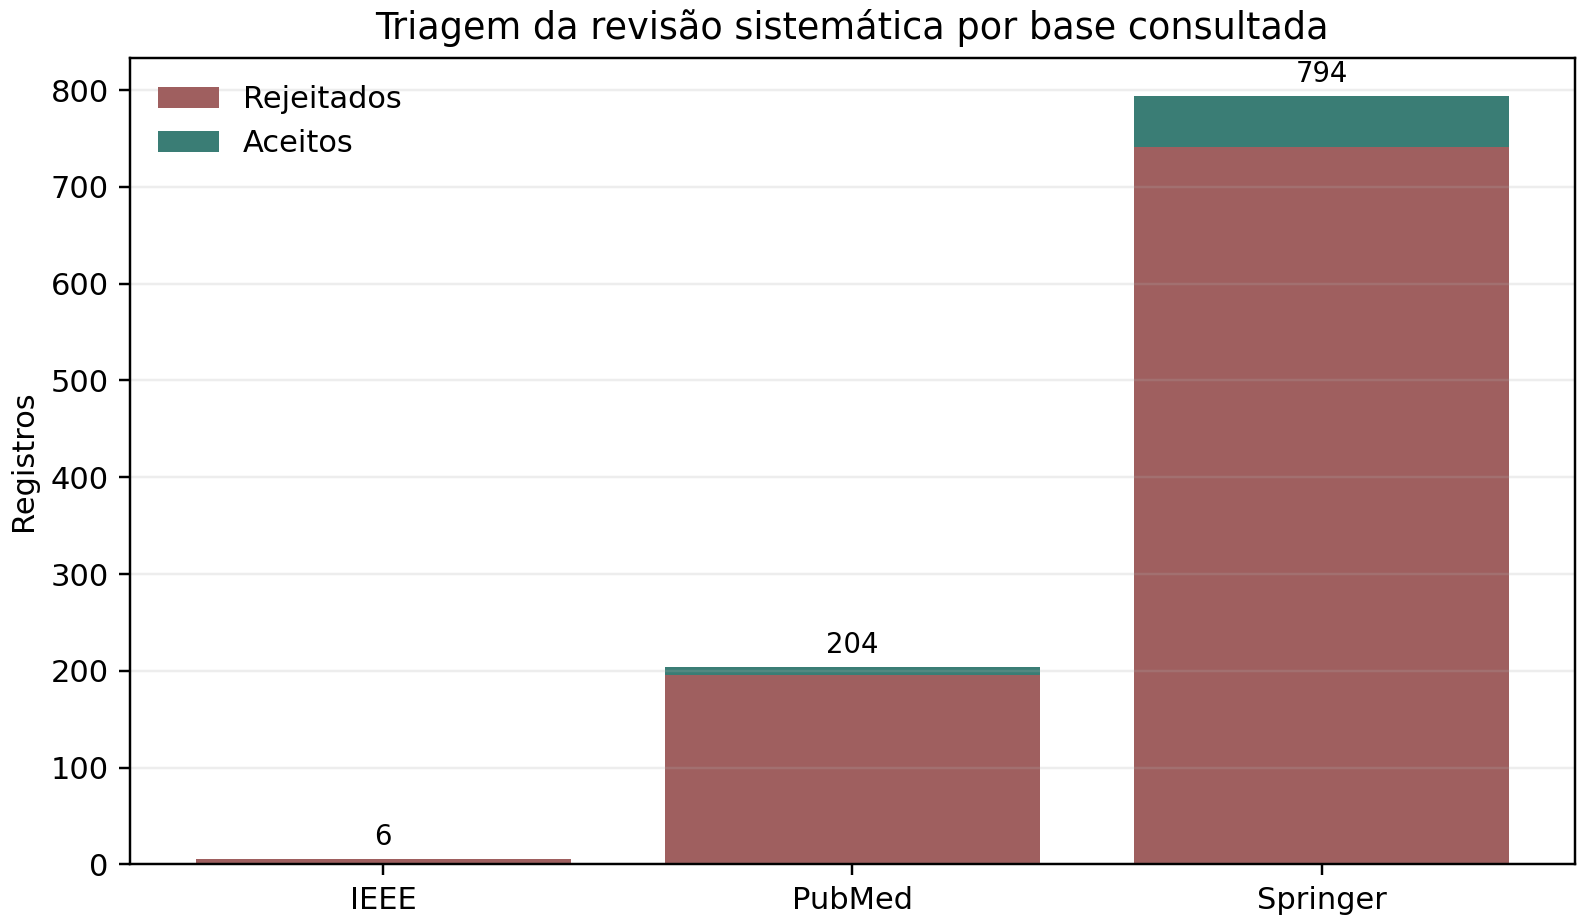
\includegraphics[width=0.88\textwidth]{figuras/systematic_review_screening.png}
    \caption[Triagem da revisão bibliográfica estruturada]{Distribuição dos
    registros aceitos e rejeitados por base consultada.}
    \label{fig:revisao-literatura-triagem}
\end{figure}

A matriz de extração apresentada no
Apêndice~\ref{ap:matriz_revisao_sistematica} registra, para cada estudo aceito,
os campos usados na síntese: referência, ano, estratégia de controle de
qualidade ou tratamento de artefatos, política de normalização, política de
particionamento, mecanismos de armazenamento e governança, uso de
\textit{ensemble} ou pós-processamento, disponibilidade de código e observações
metodológicas relevantes. A partir dessa matriz, os resultados da revisão são
organizados a seguir em torno das quatro perguntas de pesquisa definidas na
\Tabela{tab:revisao_sistematica_perguntas}. Essa organização evita uma
enumeração artigo a artigo e permite discutir, para cada pergunta, a frequência
das práticas observadas, sua função metodológica e sua relação com as decisões
adotadas nesta dissertação.

A RQ1 examinou como os estudos tratam controle de qualidade, artefatos de
lâmina, contaminação por fundo e necrose antes da extração de amostras para
aprendizagem profunda. Entre os estudos aceitos, 48 foram classificados como
contendo controle de qualidade ou tratamento explícito de artefatos, e 11
trataram a separação entre tecido e fundo como etapa operacional do fluxo. Esses
resultados reforçam a decisão de manter detecção de artefatos, triagem visual e
filtragem de regiões não informativas como fronteiras explícitas do fluxo
experimental proposto.

A RQ2 investigou como a literatura aborda particionamento, separação por
paciente e risco de vazamento de dados, inclusive em etapas de pré-processamento.
Nesse eixo, 29 estudos declararam separação por paciente. A normalização de cor,
por sua vez, foi codificada separadamente, pois atua sobre variações de
coloração, mas não substitui o isolamento entre pacientes; 33 estudos
mencionaram alguma forma de normalização. Assim, particionamento e normalização
são interpretados como controles complementares: o primeiro protege a avaliação
contra dependência entre amostras, enquanto o segundo reduz variações associadas
à aquisição e ao preparo histológico.

A RQ3 avaliou a presença de contratos explícitos de dados, orquestração,
proveniência e governança experimental. Para essa pergunta, foram considerados
sinais como repositório público, manifestos, formatos persistentes, contratos de
dados e execução orquestrada. Ao todo, 56 estudos apresentaram pelo menos um
desses elementos. Esse resultado não significa que todos os trabalhos ofereçam o
mesmo nível de auditabilidade, mas indica que parte expressiva da literatura já
registra algum vínculo verificável entre dados, código, metadados e execução.

A RQ4 analisou estratégias de agregação de modelos, incerteza e
pós-processamento, com atenção à forma como a receita final de inferência é
definida e avaliada. Nesse eixo, 27 estudos discutiram \textit{ensemble} ou
incerteza, enquanto 7 enfatizaram procedimentos de pós-processamento. Para esta
dissertação, a implicação é metodológica: qualquer receita final de
\textit{ensemble} deve ser otimizada apenas no conjunto de validação, congelada
antes da avaliação em teste e descrita como parte rastreável do protocolo, em
vez de aparecer como uma decisão genérica ou posterior aos resultados.

Em conjunto, as respostas a RQ1--RQ4 mostram que a validade de fluxos de
patologia digital oncológica depende de decisões distribuídas ao longo de todo o
processo experimental, e não apenas da arquitetura neural empregada. As
contagens apresentadas em cada pergunta derivam da classificação registrada na
matriz de extração, enquanto a classificação individual de cada estudo permanece
disponível no Apêndice~\ref{ap:matriz_revisao_sistematica}. 
